% !TEX root = ../pdf/lsr.tex
% [There are multiple lsr.tex files, but the one in ../pdf is the usual one]


\chapter{Additional \R\ concepts~\label{ch:mechanics}}

%\begin{quote}
%{\it Form follows function} \\
%\hspace*{2cm} -- Louis Sullivan
%\end{quote}

In Chapter~\ref{ch:introR} our main goal was to get started in \R. As we go through the book we'll run into a lot of new  \R\ concepts, which I'll explain alongside the relevant data analysis concepts. However, there's still quite a few things that I need to talk about now, otherwise we'll run into problems when we start trying to work with data and do statistics. So that's the goal in this chapter: to build on the introductory content from the last chapter, to get you to the point that we can start using \R\ for statistics. Broadly speaking, the chapter comes in two parts. The first half of the chapter is devoted to the ``mechanics'' of \R: installing and loading packages, managing the workspace, navigating the file system, and loading and saving data. In the second half, I'll talk more about what kinds of variables exist in \R, and introduce three new kinds of variables: factors, data frames and formulas. I'll finish up by talking a little bit about the help documentation in \R\ as well as some other avenues for finding assistance. In general, I'm not trying to be comprehensive in this chapter, I'm trying to make sure that you've got the basic foundations needed to tackle the content that comes later in the book. However, a lot of the topics are revisited in more detail later, especially in Chapters~\ref{ch:datahandling} and~\ref{ch:scripting}. 

\section{Using comments~\label{sec:comments}}

Before discussing any of the more complicated stuff, I want to introduce the \keyterm{comment} character, \rtextverb`#`. It has a simple meaning: it tells \R\ to ignore everything else you've written on this line. You won't have much need of the \rtextverb`#` character immediately, but it's very useful later on when writing scripts (see Chapter~\ref{ch:scripting}). However, while you don't need to use it, I want to be able to include comments in my \R\ extracts. For instance, if you read this:\FOOTNOTE{Notice that I used \rtextsmall{print(keeper)} rather than just typing \rtextsmall{keeper}. Later on in the text I'll sometimes use the \rtextsmall{print()} function to display things because I think it helps make clear what I'm doing, but in practice people rarely do this.}
\begin{rblock1}
> @usr{seeker <- 3.1415}           # create the first variable
> @usr{lover <- 2.7183}            # create the second variable
> @usr{keeper <- seeker * lover}   # now multiply them to create a third one
> @usr{print( keeper )}            # print out the value of 'keeper'
[1] 8.539539
\end{rblock1}
it's a lot easier to understand what I'm doing than if I just write this:
\begin{rblock1}
> @usr{seeker <- 3.1415}
> @usr{lover <- 2.7183}
> @usr{keeper <- seeker * lover}
> @usr{print( keeper )}    
[1] 8.539539
\end{rblock1}
So, from now on, you'll start seeing some \rtextverb`#` characters appearing in the extracts, with some human-readable explanatory remarks next to them. These are still perfectly legitimate commands, since \R\ knows that it should ignore the \rtextverb`#` character and everything after it. But hopefully they'll help make things a little easier to understand.

\section{Installing and loading packages~\label{sec:packageinstall}}


In this section I discuss \R\ \keyterm{packages}, since almost all of the functions you might want to use in \R\ come in packages. A package is basically just a big collection of functions, data sets and other \R\ objects that are all grouped together under a common name. Some packages are already installed when you put \R\ on your computer, but the vast majority of them of \R\ packages are out there on the internet, waiting for you to download, install and use them. 

When I first started writing this book, Rstudio didn't really exist as a viable option for using \R, and as a consequence I wrote a very lengthy section that explained how to do package management using raw \R\ commands. It's not actually terribly hard to work with packages that way, but it's clunky and unpleasant. Fortunately, we don't have to do things that way anymore. In this section, I'll describe how to work with packages using the Rstudio tools, because they're so much simpler. Along the way, you'll see that whenever you get Rstudio to do something (e.g., install a package), you'll actually see the \R\ commands that get created. I'll explain them as we go, because I think that helps you understand what's going on. 

However, before we get started, there's a critical distinction that you need to understand, which is the difference between having a package \keyterm{installed} on your computer, and having a package \keyterm{loaded} in \R. As of this writing, there are just over 5000 \R\ packages freely available ``out there'' on the internet.\FOOTNOTE{More precisely, there are 5000 or so packages on CRAN, the Comprehensive R Archive Network.} When you install \R\ on your computer, you don't get all of them: only about 30 or so come bundled with the basic \R\ installation. So right now there are about 30 packages ``installed'' on your computer, and another 5000 or so that are not installed. So that's what installed means: it means ``it's on your computer somewhere''. The critical thing to remember is that just because something is on your computer doesn't mean \R\ can use it. In order for \R\ to be able to {\it use} one of your 30 or so installed packages, that package must also be ``loaded''. Generally, when you open up \R, only a few of these packages (about 7 or 8) are actually loaded. Basically what it boils down to is this:
\begin{quote}
A package must be installed before it can be loaded.\\
A package must be loaded before it can be used.
\end{quote}
This two step process might seem a little odd at first, but the designers of \R\ had very good reasons to do it this way,\FOOTNOTE{Basically, the reason is that there are 5000 packages, and probably about 4000 authors of packages, and no-one really knows what all of them do. Keeping the installation separate from the loading minimizes the chances that two packages will interact with each other in a nasty way.} and you get the hang of it pretty quickly.


\SUBSECTION{The package panel in Rstudio}

\begin{figure}[t]
\begin{center}
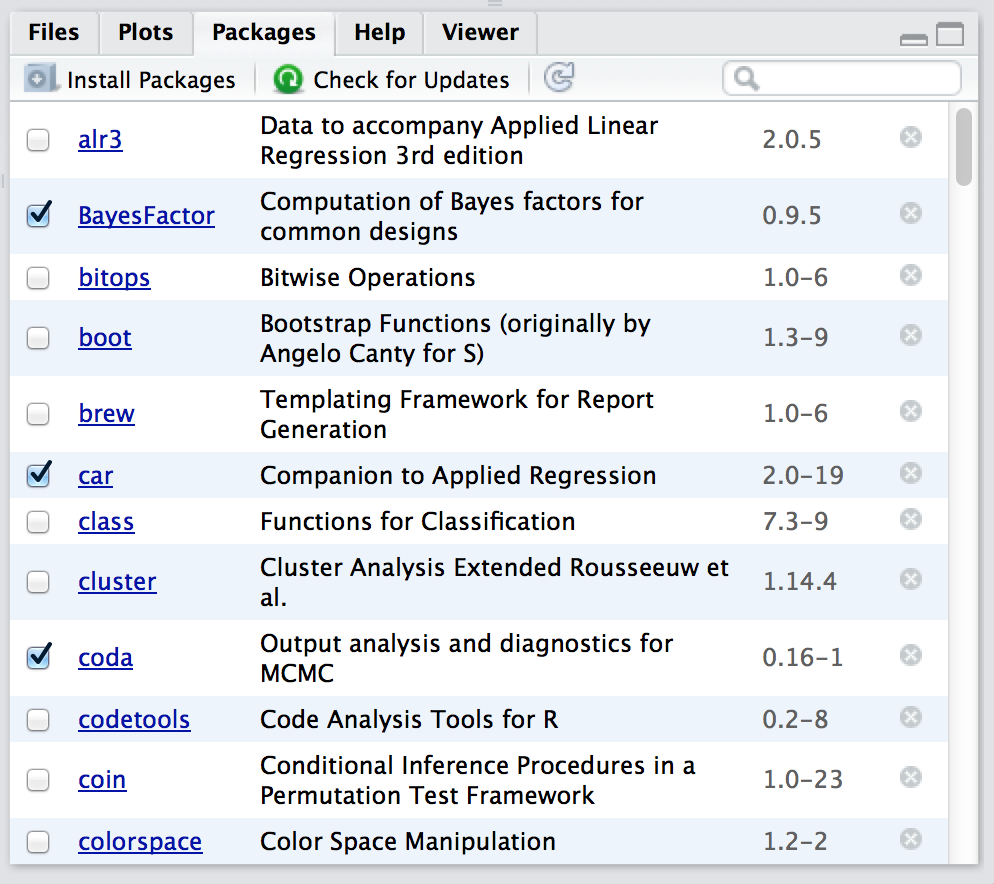
\epsfig{file=../img/mechanics/Rstudiopackages.eps,clip=true,width=10cm}
\caption{The packages panel.}
\HR
\label{fig:packagepanel}
\end{center}
\end{figure}

Right, lets get started. The first thing you need to do is look in the lower right hand panel in Rstudio. You'll see a tab labelled ``Packages''. Click on the tab, and you'll see a list of packages that looks something like Figure~\ref{fig:packagepanel}. Every row in the panel corresponds to a different package, and every column is a useful piece of information about that package.\FOOTNOTE{If you're using the command line, you can get the same information by typing \rtextsmall{library()} at the command line.} Going from left to right, here's what each column is telling you:

\begin{itemize}
\item The check box on the far left column indicates whether or not the package is loaded.
\item The one word of text immediately to the right of the check box is the name of the package.
\item The short passage of text next to the name is a brief description of the package.
\item The number next to the description tells you what version of the package you have installed.
\item The little x-mark next to the version number is a button that you can push to uninstall the package from your computer (you almost never need this).
\end{itemize}

\SUBSECTION{Loading a package\label{sec:packageload}}

That seems straightforward enough, so let's try loading and unloading packades. For this example, I'll use the \rtext{foreign} package. The \rtext{foreign} package is a collection of tools that are very handy when \R\ needs to interact with files that are produced by other software packages (e.g., SPSS). It comes bundled with \R, so it's one of the ones that you have installed already, but it won't be one of the ones loaded. Inside the \rtext{foreign} package is a function called \rtext{read.spss()}. It's a handy little function that you can use to import an SPSS data file into \R, so let's pretend we want to use it. Currently, the \rtext{foreign} package isn't loaded, so if I ask \R\ to tell me if it knows about a function called \rtext{read.spss()} it tells me that there's no such thing...
\begin{rblock1}
> @usr{exists( "read.spss" )}
[1] FALSE 
\end{rblock1}
Now let's load the package. In Rstudio, the process is dead simple: go to the package tab, find the entry for the \rtext{foreign} package, and check the box on the left hand side. The moment that you do this, you'll see a command like this appear in the \R\ console:
\begin{rblock1}
> @usr{library("foreign", lib.loc="/Library/Frameworks/R.framework/Versions/3.0/Resources/library")}
\end{rblock1}
The \rtext{lib.loc} bit will look slightly different on Macs versus on Windows, because that part of the command is just Rstudio telling \R\ where to look to find the installed packages. What I've shown you above is the Mac version. On a Windows machine, you'll probably see something that looks like this:
\begin{rblock1}
> @usr{library("foreign", lib.loc="C:/Program Files/R/R-3.0.2/library")}
\end{rblock1}
But actually it doesn't matter much. The \rtext{lib.loc} bit is almost always unnecessary. Unless you've taken to installing packages in idiosyncratic places (which is something that you can do if you really want) \R\ already knows where to look. So in the vast majority of cases, the command to load the \rtext{foreign} package is just this:
\begin{rblock1}
> @usr{library("foreign")}
\end{rblock1}
Throughout this book, you'll often see me typing in \rtext{library()} commands. You don't actually have to type them in yourself: you can use the Rstudio package panel to do all your package loading for you. The only reason I include the \rtext{library()} commands sometimes is as a reminder to you to make sure that you have the relevant package loaded. Oh, and I suppose we should check to see if our attempt to load the package actually worked. Let's see if \R\ now knows about the existence of the \rtext{read.spss()} function...
\begin{rblock1}
> @usr{exists( "read.spss" )}
[1] TRUE 
\end{rblock1}
Yep. All good.



\SUBSECTION{Unloading a package\label{sec:packageunload}}


Sometimes, especially after a long session of working with \R, you find yourself wanting to get rid of some of those packages that you've loaded. The Rstudio package panel makes this exactly as easy as loading the package in the first place. Find the entry corresponding to the package you want to unload, and uncheck the box. When you do that for the \rtext{foreign} package, you'll see this command appear on screen:
\begin{rblock1}
> @usr{detach("package:foreign", unload=TRUE)}
\end{rblock1}
And the package is unloaded. We can verify this by seeing if the \rtext{read.spss()} function still \rtext{exists()}: 
\begin{rblock1}
> @usr{exists( "read.spss" )}
[1] FALSE 
\end{rblock1}
Nope. Definitely gone. 



\SUBSECTION{A few extra comments}

Sections~\ref{sec:packageload} and \ref{sec:packageunload} cover the main things you need to know about loading and unloading packages. However, there's a couple of other details that I want to draw your attention to. A concrete example is the best way to illustrate. One of the other packages that you already have installed on your computer is the \rtext{Matrix} package, so let's load that one and see what happens:
\begin{rblock1}
> @usr{library( Matrix )}
Loading required package: lattice
\end{rblock1}
This is slightly more complex than the output that we got last time, but it's not too complicated. The \rtext{Matrix} package makes use of some of the tools in the \rtext{lattice} package, and \R\ has kept track of this dependency. So when you try to load the \rtext{Matrix} package, \R\ recognises that you're also going to need to have the \rtext{lattice} package loaded too. As a consequence, {\it both} packages get loaded, and \R\ prints out a helpful little note on screen to tell you that it's done so. 

\R\ is pretty aggressive about enforcing these dependencies. Suppose, for example, I try to unload the \rtext{lattice} package while the \rtext{Matrix} package is still loaded. This is easy enough to try: all I have to do is uncheck the box next to ``lattice'' in the packages panel. But if I try this, here's what happens:
\begin{rblock1}
> @usr{detach("package:lattice", unload=TRUE)}
Error: package `lattice' is required by `Matrix' so will not be detached
\end{rblock1}
\R\ refuses to do it. This can be quite useful, since it stops you from accidentally removing something that you still need. So, if I want to remove both \rtext{Matrix} and \rtext{lattice}, I need to do it in the correct order


Something else you should be aware of. Sometimes you'll attempt to load a package, and \R\ will print out a message on screen telling you that something or other has been ``masked''. This will be confusing to you if I don't explain it now, and it actually ties very closely to the whole reason why \R\ forces you to load packages separately from installing them. Here's an example. Two of the package that I'll refer to a lot in this book are called \rtext{car} and \rtext{psych}. The \rtext{car} package is short for ``Companion to Applied Regression'' (which is a really great book, I'll add), and it has a lot of tools that I'm quite fond of. The \rtext{car} package was written by a guy called John Fox, who has written a lot of great statistical tools for social science applications. The \rtext{psych} package was written by William Revelle, and it has a lot of functions that are very useful for psychologists in particular, especially in regards to psychometric techniques. For the most part, \rtext{car} and \rtext{psych} are quite unrelated to each other. They do different things, so not surprisingly almost all of the function names are different. But... there's one exception to that. The \rtext{car} package and the \rtext{psych} package {\it both} contain a function called \rtext{logit()}.\FOOTNOTE{The logit function a simple mathematical function that happens not to have been included in the basic \R\ distribution.} This creates a naming conflict. If I load both packages into \R, an ambiguity is created. If the user types in \rtext{logit(100)}, should \R\ use the \rtext{logit()} function in the \rtext{car} package, or the one in the \rtext{psych} package? The answer is: \R\ uses whichever package you loaded most recently, and it tells you this very explicitly. Here's what happens when I load the \rtext{car} package, and then afterwards load the \rtext{psych} package: 
\begin{rblock1}
> @usr{library(car)}
> @usr{library(psych)}
Attaching package: `psych'

The following object is masked from `package:car':

    logit
\end{rblock1}
The output here is telling you that the \rtext{logit} object (i.e., function) in the \rtext{car} package is no longer accessible to you. It's been hidden (or ``masked'') from you by the one in the \rtext{psych} package.\FOOTNOTE{Tip for advanced users. You can get \R\ to use the one from the \rtextsmall{car} package by using \rtextsmall{car::logit()} as your command rather than \rtextsmall{logit()}, since the \rtextsmall{car::} part tells \R\ explicitly which package to use. See also \rtextsmall{:::} if you're especially keen to force \R\ to use functions it otherwise wouldn't, but take care, since \rtextsmall{:::} can be dangerous.}

\SUBSECTION{Downloading new packages}

One of the main selling points for \R\ is that there are thousands of packages that have been written for it, and these are all available online. So whereabouts online are these packages to be found, and how do we download and install them?  There is a big repository of packages called the ``Comprehensive R Archive Network'' (CRAN), and the easiest way of getting and installing a new package is from one of the many CRAN mirror sites. Conveniently for us, \R\ provides a function called \rtext{install.packages()} that you can use to do this. Even {\it more} conveniently, the Rstudio team runs its own CRAN mirror and Rstudio has a clean interface that lets you install packages without having to learn how to use the \rtext{install.packages()} command\FOOTNOTE{It is not very difficult.}

Using the Rstudio tools is, again, dead simple. In the top left hand corner of the packages panel (Figure~\ref{fig:packagepanel}) you'll see a button called ``Install Packages''. If you click on that, it will bring up a window like the one shown in Figure~\ref{fig:packageinstall}a. There are a few different buttons and boxes you can play with. Ignore most of them. Just go to the line that says ``Packages'' and start typing the name of the package that you want. As you type, you'll see a dropdown menu appear (Figure~\ref{fig:packageinstall}b), listing names of packages that start with the letters that you've typed so far. You can select from this list, or just keep typing. Either way, once you've got the package name that you want, click on the install button at the bottom of the window. When you do, you'll see the following command appear in the \R\ console:
\begin{rblock1}
> @usr{install.packages("psych")}
\end{rblock1}
This is the \R\ command that does all the work. \R\ then goes off to the internet, has a conversation with CRAN, downloads some stuff, and installs it on your computer. You probably don't care about all the details of \R's little adventure on the web, but the \rtext{install.packages()} function is rather chatty, so it reports a bunch of gibberish that you really aren't all that interested in:
\begin{rblock1}
trying URL 'http://cran.rstudio.com/bin/macosx/contrib/3.0/psych_1.4.1.tgz'
Content type 'application/x-gzip' length 2737873 bytes (2.6 Mb)
opened URL
==================================================
downloaded 2.6 Mb


The downloaded binary packages are in
	/var/folders/cl/thhsyrz53g73q0w1kb5z3l_80000gn/T//RtmpmQ9VT3/downloaded_packages
\end{rblock1}
Despite the long and tedious response, all thar really means is ``I've installed the psych package''. I find it best to humour the talkative little automaton. I don't actually read any of this garbage, I just politely say ``thanks'' and go back to whatever I was doing.  


\begin{figure}[t]
\begin{center}
\begin{tabular}{ccc}
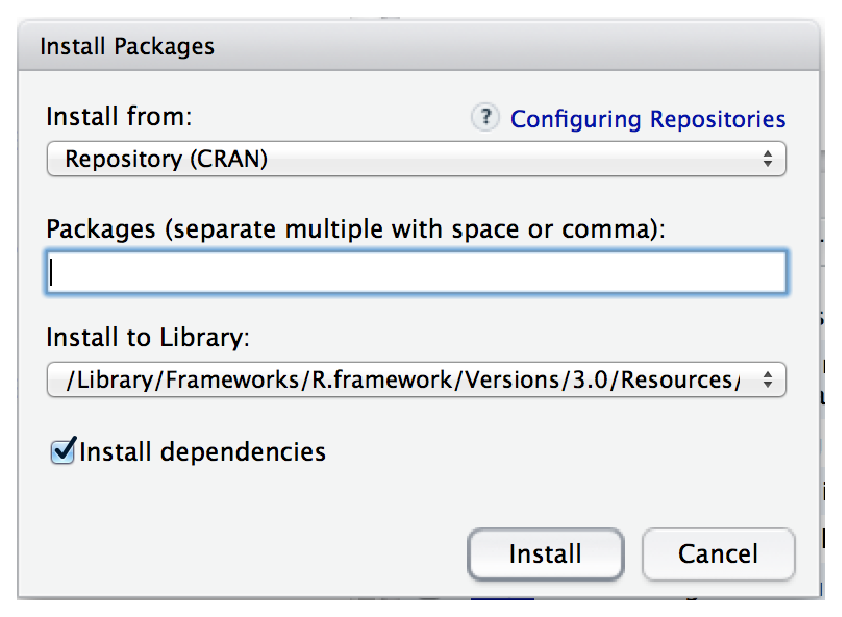
\epsfig{file = ../img/mechanics/installpackage.eps, clip=true,width = 7cm} & \hspace{.5cm} &
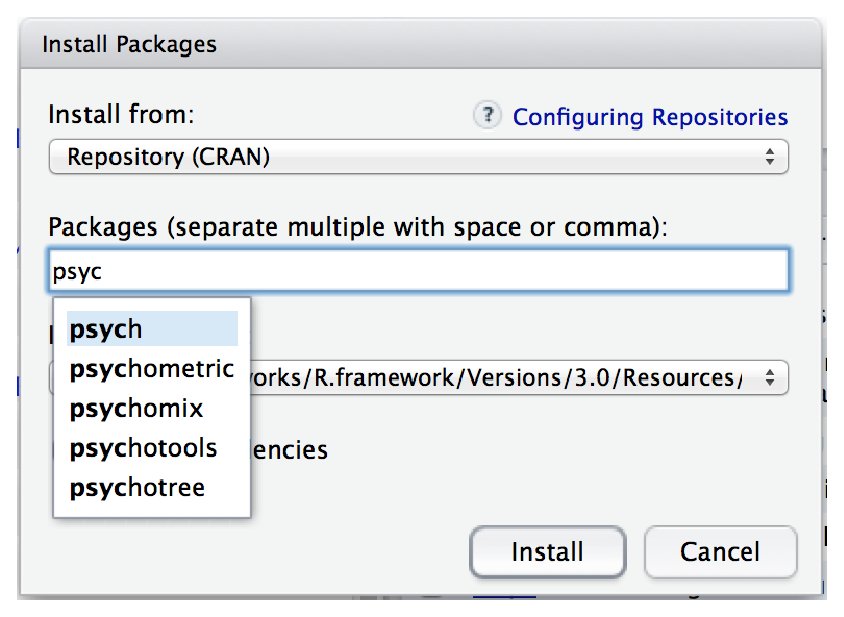
\epsfig{file = ../img/mechanics/installpackage2.eps,clip=true, width = 7cm} \\
(a) && (b)
\end{tabular}
\caption{The package installation dialog box in Rstudio (panel a). When you start typing, you'll see a dropdown menu suggest a list of possible packages that you might want to install (panel b)}
\HR
\label{fig:packageinstall}
\end{center}
\end{figure}



\SUBSECTION{Updating \R\ and \R\ packages}

Every now and then the authors of packages release updated versions. The updated versions often add new functionality, fix bugs, and so on. It's generally a good idea to update your packages periodically. There's an \rtext{update.packages()} function that you can use to do this, but it's probably easier to stick with the Rstudio tool. In the packages panel, click on the ``Update Packages'' button. This will bring up a window that looks like the one shown in Figure~\ref{fig:updatepackages}. In this window, each row refers to a package that needs to be updated. You can to tell \R\ which updates you want to install by checking the boxes on the left. If you're feeling lazy and just want to update everything, click the ``Select All'' button, and then click the ``Install Updates'' button. \R\ then prints out a {\it lot} of garbage on the screen, individually downloading and installing all the new packages. This might take a while to complete depending on how good your internet connection is. Go make a cup of coffee. Come back, and all will be well. 

\begin{figure}[t]
\begin{center}
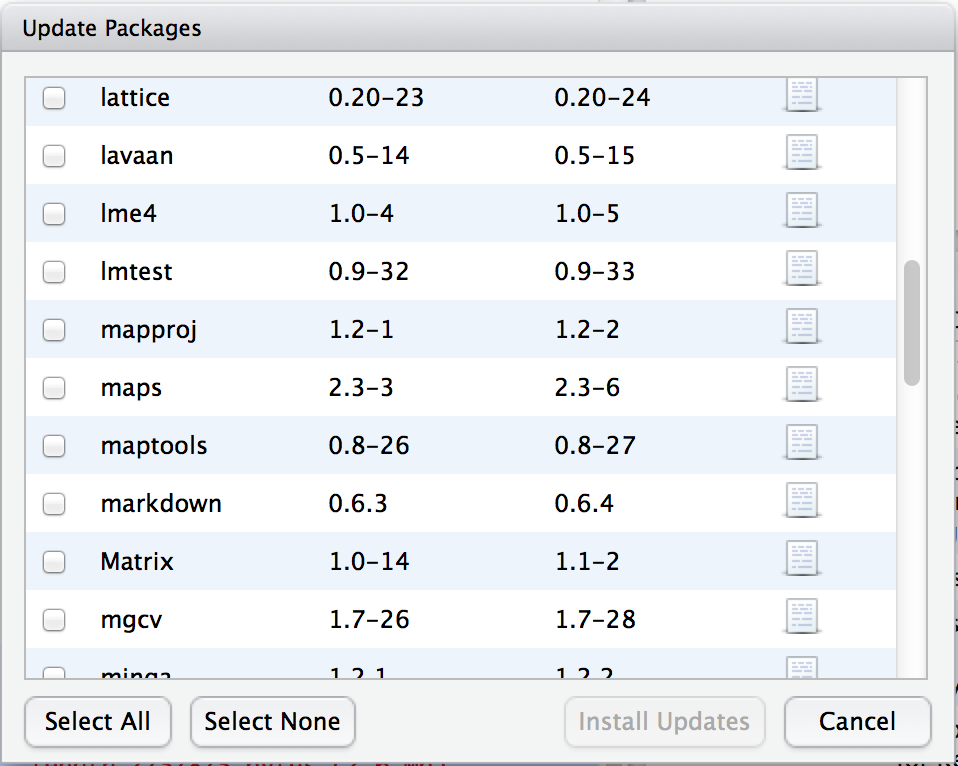
\epsfig{file=../img/mechanics/updatepackages.eps,clip=true,width=10cm}
\caption{The Rstudio dialog box for updating packages.}
\HR
\label{fig:updatepackages}
\end{center}
\end{figure}


About every six months or so, a new version of \R\ is released. You can't update \R\ from within Rstudio (not to my knowledge, at least): to get the new version you can go to the CRAN website and download the most recent version of \R, and install it in the same way you did when you originally installed \R\ on your computer. This used to be a slightly frustrating event, because whenever you downloaded the new version of \R, you would lose all the packages that you'd downloaded and installed, and would have to repeat the process of re-installing them. This was pretty annoying, and there were some neat tricks you could use to get around this. However, newer versions of \R\ don't have this problem so I no longer bother explaining the workarounds for that issue.

\SUBSECTION{What packages does this book use?}


There are several packages that I make use of in this book. The most prominent ones are:

\begin{itemize}
\item \rtext{lsr}. This is the {\it Learning Statistics with R} package that accompanies this book. It doesn't have a lot of interesting high-powered tools: it's just a small collection of handy little things that I think can be useful to novice users. As you get more comfortable with \R\ this package should start to feel pretty useless to you.
\item \rtext{psych}. This package, written by William Revelle, includes a lot of tools that are of particular use to psychologists. In particular, there's several functions that are particularly convenient for producing analyses or summaries that are very common in psych, but less common in other disciplines. 
\item \rtext{car}. This is the {\it Companion to Applied Regression} package, which accompanies the excellent book of the same name by \citeA{Fox2011}. It provides a lot of very powerful tools, only some of which we'll touch in this book.
\end{itemize}

\noindent 
Besides these three, there are a number of packages that I use in a more limited fashion: \rtext{gplots}, \rtext{sciplot}, \rtext{foreign},  \rtext{effects}, \rtext{R.matlab}, \rtext{gdata}, \rtext{lmtest}, and probably one or two others that I've missed. There are also a number of packages that I refer to but don't actually use in this book, such as \rtext{reshape}, \rtext{compute.es}, \rtext{HistData} and \rtext{multcomp} among others. Finally, there are a number of packages that provide more advanced tools that I hope to talk about in future versions of the book, such as \rtext{sem}, \rtext{ez}, \rtext{nlme} and \rtext{lme4}. In any case, whenever I'm using a function that isn't in the core packages, I'll make sure to note this in the text.



\section{Managing the workspace\label{sec:workspace}}

Let's suppose that you're reading through this book, and what you're doing is sitting down with it once a week and working through a whole chapter in each sitting. Not only that, you've been following my advice and typing in all these commands into \R. So far during this chapter, you'd have typed quite a few commands, although the only ones that actually involved creating variables were the ones you typed during Section~\ref{sec:comments}. As a result, you currently have three variables; \rtext{seeker}, \rtext{lover}, and \rtext{keeper}. These three variables are the contents of your \keyterm{workspace}, also referred to as the \textbf{global environment}. The workspace is a key concept in \R, so in this section we'll talk a lot about what it is and how to manage its contents.



\SUBSECTION{Listing the contents of the workspace}


\begin{figure}[t]
\begin{center}
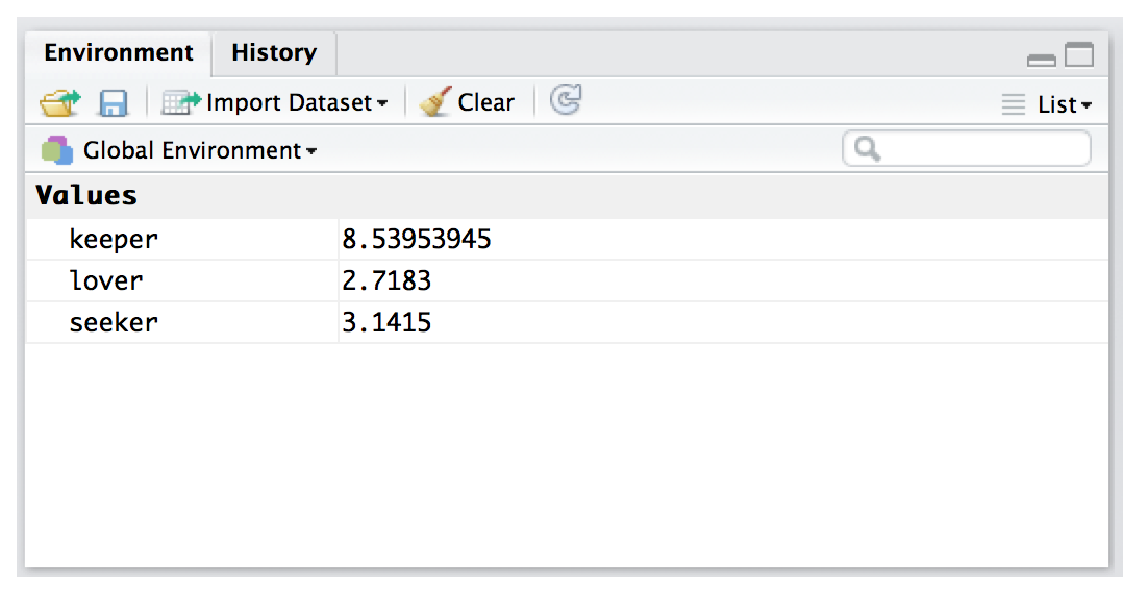
\epsfig{file=../img/mechanics/workspacepanel.eps,clip=true,width=10cm}
\caption{The Rstudio ``Environment'' panel shows you the contents of the workspace. The view shown above is the ``list'' view. To switch to the grid view, click on the menu item on the top right that currently reads ``list''. Select ``grid'' from the dropdown menu, and then it will switch to a view like the one shown in Figure~\protect\ref{fig:workspace2}.}
\HR
\label{fig:workspace}
\end{center}
\end{figure}

\begin{figure}[t]
\begin{center}
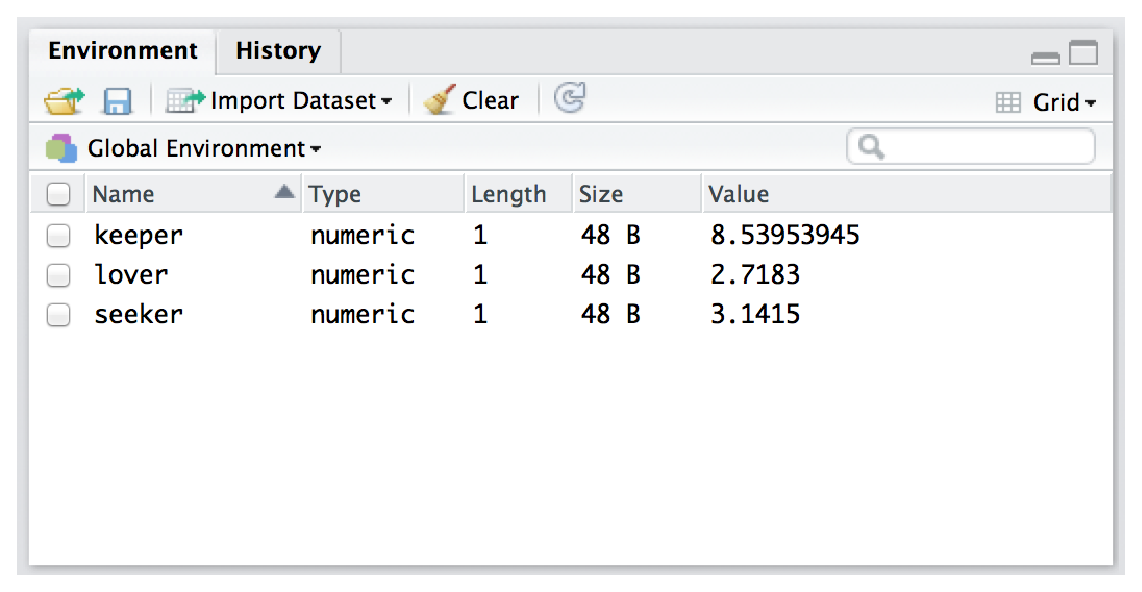
\epsfig{file=../img/mechanics/workspacepanel2.eps,clip=true,width=10cm}
\caption{The Rstudio ``Environment'' panel shows you the contents of the workspace. Compare this ``grid'' view to the ``list'' view in Figure~\protect\ref{fig:workspace}}
\HR
\label{fig:workspace2}
\end{center}
\end{figure}


The first thing that you need to know how to do is examine the contents of the workspace. If you're using Rstudio, you will probably find that the easiest way to do this is to use the ``Environment'' panel in the top right hand corner. Click on that, and you'll see a list that looks very much like the one shown in Figures~\ref{fig:workspace} and \ref{fig:workspace2}.  If you're using the commmand line, then the \rtext{objects()} function may come in handy:
\begin{rblock1}
> @usr{objects()}
[1] "keeper" "lover"  "seeker"
\end{rblock1}
Of course, in the true \R\ tradition, the \rtext{objects()} function has a lot of fancy capabilities that I'm glossing over in this example. Moreover there are also several other functions that you can use, including \rtext{ls()} which is pretty much identical to \rtext{objects()}, and \rtext{ls.str()} which you can use to get a fairly detailed description of all the variables in the workspace. In fact, the \rtext{lsr} package actually includes its own function that you can use for this purpose, called \rtext{who()}. The reason for using the \rtext{who()} function is pretty straightforward: in my everyday work I find that the output produced by the \rtext{objects()} command isn't {\it quite} informative enough, because the only thing it prints out is the name of each variable; but the \rtext{ls.str()} function is {\it too} informative, because it prints out a lot of additional information that I really don't like to look at. The \rtext{who()} function is a compromise between the two. First, now that we've got the \rtext{lsr} package installed, we need to load it:
\begin{rblock1}
> @usr{library(lsr)}
\end{rblock1}
and now we can use the \rtext{who()} function:
\begin{rblock1}
> @usr{who()}
   -- Name --   -- Class --   -- Size --
   keeper       numeric       1         
   lover        numeric       1         
   seeker       numeric       1         
\end{rblock1}
As you can see, the \rtext{who()} function lists all the variables and provides some basic information about what kind of variable each one is and how many elements it contains. Personally, I find this output much easier more useful than the very compact output of the \rtext{objects()} function, but less overwhelming than the extremely verbose \rtext{ls.str()} function. Throughout this book you'll see me using the \rtext{who()} function a lot. You don't have to use it yourself: in fact, I suspect you'll find it easier to look at the Rstudio environment panel. But for the purposes of writing a textbook I found it handy to have a nice text based description: otherwise there would be about another 100 or so screenshots added to the book.\FOOTNOTE{This would be especially annoying if you're reading an electronic copy of the book because the text displayed by the \rtextsmall{who()} function is searchable, whereas text shown in a screen shot isn't!}


\SUBSECTION{Removing variables from the workspace}

Looking over that list of variables, it occurs to me that I really don't need them any more. I created them originally just to make a point, but they don't serve any useful purpose anymore, and now I want to get rid of them.  I'll show you how to do this, but first I want to warn you -- there's no ``undo'' option for variable removal. Once a variable is removed, it's gone forever unless you save it to disk. I'll show you how to do {\it that} in Section~\ref{sec:load}, but quite clearly we have no need for these variables at all, so we can safely get rid of them.

In Rstudio, the easiest way to remove variables is to use the environment panel. Assuming that you're in grid view (i.e., Figure~\ref{fig:workspace2}), check the boxes next to the variables that you want to delete, then click on the ``Clear'' button at the top of the panel. When you do this, Rstudio will show a dialog box asking you to confirm that you really do want to delete the variables. It's always worth checking that you really do, because as Rstudio is at pains to point out, you can't undo this. Once a variable is deleted, it's gone.\FOOTNOTE{Mind you, all that means is that it's been removed from the workspace. If you've got the data saved to file somewhere, then that {\it file} is perfectly safe.} In any case, if you click ``yes'', that variable will disappear from the workspace: it will no longer appear in the environment panel, and it won't show up when you use the \rtext{who()} command.

Suppose you don't access to Rstudio, and you still want to remove variables. This is where the \keyterm{remove} function \rtext{rm()} comes in handy. The simplest way to use \rtext{rm()} is just to type in a (comma separated) list of all the variables you want to remove. Let's say I want to get rid of \rtext{seeker} and \rtext{lover}, but I would like to keep \rtext{keeper}. To do this, all I have to do is type:
\begin{rblock1}
> @usr{rm( seeker, lover )}
\end{rblock1}
There's no visible output, but if I now inspect the workspace
\begin{rblock1}
> @usr{who()}
   -- Name --   -- Class --   -- Size --
   keeper       numeric       1         
\end{rblock1}
I see that there's only the \rtext{keeper} variable left. As you can see, \rtext{rm()} can be very handy for keeping the workspace tidy. 






\section{Navigating the file system\label{sec:navigation}}


In this section I talk a little about how \R\ interacts with the file system on your computer. It's not a terribly interesting topic, but it's useful.  As background to this discussion, I'll talk a bit about how file system locations work in Section~\ref{sec:filesystem}. Once upon a time {\it everyone} who used computers could safely be assumed to understand how the file system worked, because it was impossible to successfully use a computer if you didn't! However, modern operating systems are much more ``user friendly'', and as a consequence of this they go to great lengths to hide the file system from users. So these days it's not at all uncommon for people to have used computers most of their life and not be familiar with the way that computers organise files. If you already know this stuff, skip straight to Section~\ref{sec:navigationR}. Otherwise, read on. I'll try to give a brief introduction that will be useful for those of you who have never been forced to learn how to navigate around a computer using a DOS or UNIX shell. 

\SUBSECTION{The file system itself~\label{sec:filesystem}}

In this section I describe the basic idea behind file locations and file paths. Regardless of whether you're using Window, Mac OS or Linux, every file on the computer is assigned a (fairly) human readable address, and every address has the same basic structure: it describes a {\it path} that starts from a {\it root} location , through as series of {\it folders} (or if you're an old-school computer user, {\it directories}), and finally ends up at the file. 

On a Windows computer the root is the physical drive\FOOTNOTE{Well, the partition, technically.} on which the file is stored, and for most home computers the name of the hard drive that stores all your files is \filename{C:} and therefore most file names on Windows begin with \filename{C:}. After that comes the folders, and on Windows the folder names are separated by a \verb#\# symbol. So, the complete path to this book on my Windows computer might be something like this:
\begin{verbatim}
C:\Users\dan\Rbook\LSR.pdf
\end{verbatim}
and what that {\it means} is that the book is called \filename{LSR.pdf}, and it's in a folder called \filename{Rbook} which itself is in a folder called \filename{dan} which itself is ... well, you get the idea. On Linux, Unix and Mac OS systems, the addresses look a little different, but they're more or less identical in spirit. Instead of using the backslash, folders are separated using a forward slash, and unlike Windows, they don't treat the physical drive as being the root of the file system. So, the path to this book on my Mac might be something like this:
\begin{verbatim}
/Users/dan/Rbook/LSR.pdf
\end{verbatim}

So that's what we mean by the ``path'' to a file. The next concept to grasp is the idea of a \keyterm{working directory} and how to change it. For those of you who have used command line interfaces previously, this should be obvious already. But if not, here's what I mean. The working directory is just ``whatever folder I'm currently looking at''. Suppose that I'm currently looking for files in Explorer (if you're using Windows) or using Finder (on a Mac). The folder I currently have open is my user directory (i.e., \verb#C:\Users\dan# or \verb#/Users/dan#). That's my current working directory. 

The fact that we can imagine that the program is ``in'' a particular directory means that we can talk about moving {\it from} our current location {\it to} a new one. What that means is that we might want to specify a new location in relation to our current location. To do so, we need to introduce two new conventions. Regardless of what operating system you're using, we use \filename{.} to refer to the current working directory, and \filename{..} to refer to the directory above it. This allows us to specify a path to a new location in relation to our current location, as the following examples illustrate. Let's assume that I'm using my Windows computer, and my working directory is \verb#C:\Users\dan\Rbook#). The table below shows several addresses in relation to my current one:
\begin{center}
\begin{tabular}{l|l}
absolute path  & relative path \\ 
(i.e., from root)  & (i.e. from \verb#C:\Users\dan\Rbook#) \\[4pt] \hline \\[-12pt]
\verb#C:\Users\dan# & \verb#..# \\
\verb#C:\Users# & \verb#..\..# \\
\verb#C:\Users\dan\Rbook\source# & \verb#.\source# \\
\verb#C:\Users\dan\nerdstuff# & \verb#..\nerdstuff# \\
\end{tabular}
\end{center}


There's one last thing I want to call attention to: the \verb#~# directory. I normally wouldn't bother, but \R\ makes reference to this concept sometimes. It's quite common on computers that have multiple users to define \verb#~# to be the user's home directory. On my Mac, for instance, the home directory \verb#~# for the ``dan'' user is \verb#\Users\dan\#. And so, not surprisingly, it is possible to define other directories in terms of their relationship to the home directory. For example, an alternative way to describe the location of the \filename{LSR.pdf} file on my Mac would be 
\begin{verbatim}
~\Rbook\LSR.pdf
\end{verbatim}


That's about all you really need to know about file paths. And since this section already feels too long, it's time to look at how to navigate the file system in \R. 

\SUBSECTION{Navigating the file system using the \R\ console~\label{sec:navigationR}}

In this section I'll talk about how to navigate this file system from within \R\ itself. It's not particularly user friendly, and so you'll probably be happy to know that Rstudio provides you with an easier method, and I will describe it in Section~\ref{sec:nav3}. So in practice, you won't {\it really} need to use the commands that I babble on about in this section, but I do think it helps to see them in operation at least once before forgetting about them forever.

Okay, let's get started. When you want to load or save a file in \R\ it's important to know what the working directory is. You can find out by using the \rtext{getwd()} command. For the moment, let's assume that I'm using Mac OS or Linux, since there's some subtleties to Windows. Here's what happens:
\begin{rblock1}
> @usr{getwd()}
[1] "/Users/dan"
\end{rblock1}
We can change the working directory quite easily using \rtext{setwd()}. The \rtext{setwd()} function has only the one argument, \rtext{dir},  is a character string specifying a path to a directory, or a path relative to the working directory. Since I'm currently located at \verb#/Users/dan#, the following two are equivalent: 
\begin{rblock1}
> @usr{setwd("/Users/dan/Rbook/data")}
> @usr{setwd("./Rbook/data")}
\end{rblock1}
Now that we're here, we can type \rtext{list.files()} command to get a listing of all the files in that directory. Since this is the directory in which I store all of the data files that we'll use in this book, here's what we get as the result:
\begin{rblock1}
> @usr{list.files()}
 [1] "afl24.Rdata"             "aflsmall.Rdata"          "aflsmall2.Rdata"        
 [4] "agpp.Rdata"              "all.zip"                 "annoying.Rdata"         
 [7] "anscombesquartet.Rdata"  "awesome.Rdata"           "awesome2.Rdata"         
[10] "booksales.csv"           "booksales.Rdata"         "booksales2.csv"         
[13] "cakes.Rdata"             "cards.Rdata"             "chapek9.Rdata"          
[16] "chico.Rdata"             "clinicaltrial_old.Rdata" "clinicaltrial.Rdata"    
[19] "coffee.Rdata"            "drugs.wmc.rt.Rdata"      "dwr_all.Rdata"          
[22] "effort.Rdata"            "happy.Rdata"             "harpo.Rdata"            
[25] "harpo2.Rdata"            "likert.Rdata"            "nightgarden.Rdata"      
[28] "nightgarden2.Rdata"      "parenthood.Rdata"        "parenthood2.Rdata"      
[31] "randomness.Rdata"        "repeated.Rdata"          "rtfm.Rdata"             
[34] "salem.Rdata"             "zeppo.Rdata"
\end{rblock1}
Not terribly exciting, I'll admit, but it's useful to know about. In any case, there's only one more thing I want to make a note of, which is that \R\ also makes use of the home directory. You can find out what it is by using the \rtext{path.expand()} function, like this:
\begin{rblock1}
> @usr{path.expand("~")}
[1] "/Users/dan"
\end{rblock1}
You can change the user directory if you want, but we're not going to make use of it very much so there's no reason to. The only reason I'm even bothering to mention it at all is that when you use Rstudio to open a file, you'll see output on screen that defines the path to the file relative to  the \rtextverb#~# directory. I'd prefer you not to be confused when you see it.\FOOTNOTE{One additional thing worth calling your attention to is the \rtextsmall{file.choose()} function. Suppose you want to load a file and you don't quite remember where it is, but would like to browse for it. Typing \rtextsmall{file.choose()} at the command line will open a window in which you can browse to find the file; when you click on the file you want, \R\ will print out the full path to that file. This is kind of handy.}




\SUBSECTION{Why do the Windows paths use the wrong slash?}

Let's suppose I'm on Windows. As before, I can find out what my current working directory is like this:
\begin{rblock1}
> @usr{getwd()}
[1] "C:/Users/dan/
\end{rblock1}
This seems about right, but you might be wondering why \R\ is displaying a Windows path using the wrong type of slash. The answer is slightly complicated, and has to do with the fact that \R\ treats the \rtextverb#\# character as ``special'' (see Section~\ref{sec:escapechars}). If you're deeply wedded to the idea of specifying a path using the Windows style slashes, then what you need to do is to type \rtextverb#\\# whenever you mean \rtextverb#\#. In other words, if you want to specify the working directory on a Windows computer, you need to use one of the following commands:
\begin{rblock1}
> @usr{setwd( "C:/Users/dan" )}
> @usr{setwd( "C:\\Users\\dan" )}
\end{rblock1}
It's kind of annoying to have to do it this way, but as you'll see later on in Section~\ref{sec:escapechars} it's a necessary evil. Fortunately, as we'll see in the next section, Rstudio provides a much simpler way of changing directories...

\SUBSECTION{Navigating the file system using the Rstudio file panel\label{sec:nav3}}

Although I think it's important to understand how all this command line stuff works, in many (maybe even most) situations there's an easier way. For our purposes, the easiest way to navigate the file system is to make use of Rstudio's built in tools. The ``file'' panel -- the lower right hand area in Figure~\ref{fig:filepanel} -- is actually a pretty decent file browser. Not only can you just point and click on the names to move around the file system, you can also use it to set the working directory, and even load files. 

\begin{figure}[t]
\begin{center}
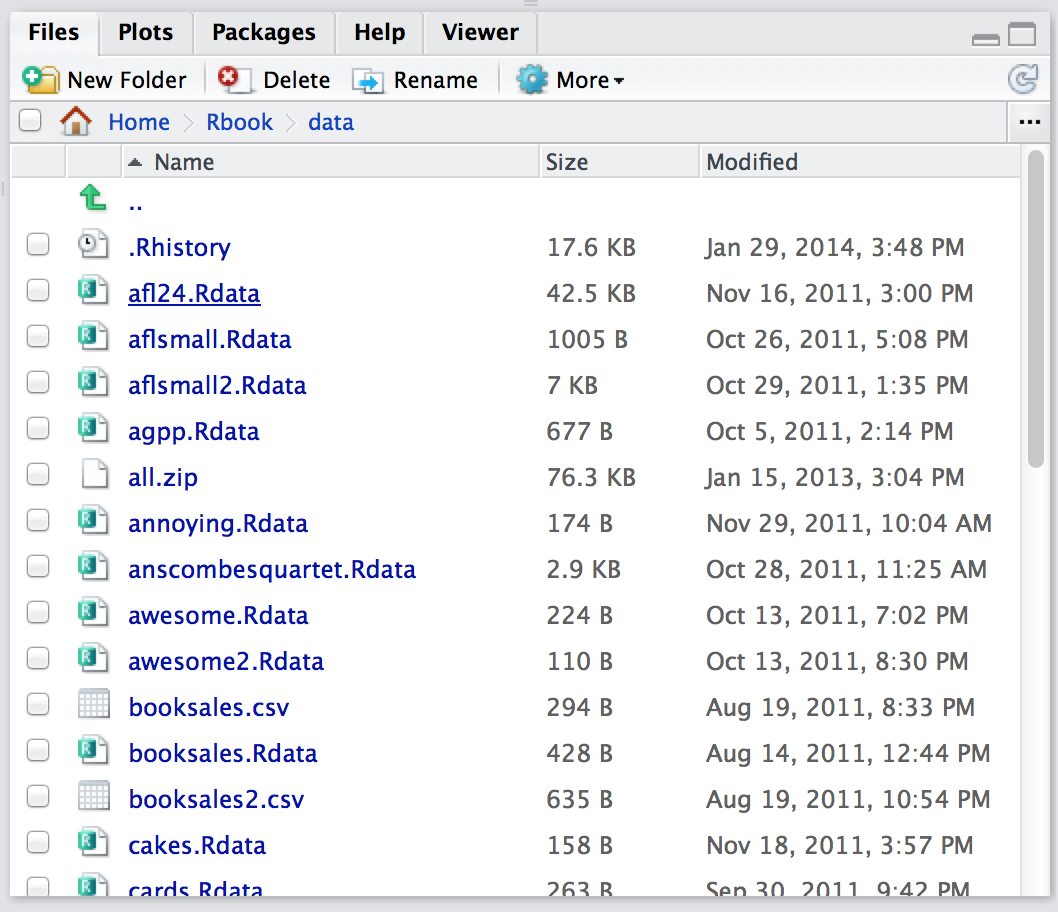
\epsfig{file=../img/mechanics/filepanel.eps,clip=true,width=10cm}
\caption{The ``file panel'' is the area shown in the lower right hand corner. It provides a very easy way to browse and navigate your computer using \R. See main text for details.}
\HR
\label{fig:filepanel}
\end{center}
\end{figure}


Here's what you need to do to change the working directory using the file panel. Let's say I'm looking at the actual screen shown in Figure~\ref{fig:filepanel}. At the top of the file panel you see some text that says ``Home $>$ Rbook $>$ data''. What that means is that it's {\it displaying} the files that are stored in the 
\begin{verbatim}
/Users/dan/Rbook/data
\end{verbatim}
directory on my computer. It does {\it not} mean that this is the \R\ working directory. If you want to change the \R\ working directory, using the file panel, you need to click on the button that reads ``More''. This will bring up a little menu, and one of the options will be ``Set as Working Directory''. If you select that option, then \R\ really will change the working directory. You can tell that it has done so because this command appears in the console: 
\begin{rblock1}
> @usr{setwd("~/Rbook/data")}
\end{rblock1}
In other words, Rstudio sends a command to the \R\ console, exactly as if you'd typed it yourself. The file panel can be used to do other things too. If you want to move ``up'' to the parent folder (e.g., from \texttt{/Users/dan/Rbook/data} to \texttt{/Users/dan/Rbook}) click on the ``..'' link in the file panel. To move to a subfolder, click on the name of the folder that you want to open. You can open some types of file by clicking on them. You can delete files from your computer using the ``delete'' button, rename them with the ``rename'' button, and so on.


As you can tell, the file panel is a very handy little tool for navigating the file system. But it can do more than just navigate. As we'll see later, it can be used to open files. And if you look at the buttons and menu options that it presents, you can even use it to rename, delete, copy or move files, and create new folders. However, since most of that functionality isn't critical to the basic goals of this book, I'll let you discover those on your own.



\section{Loading and saving data\label{sec:load}}


There are several different types of files that are likely to be relevant to us when doing data analysis. There are three in particular that are especially important from the perspective of this book:
\begin{itemize}
\item {\it Workspace files} are those with a \filename{.Rdata} file extension. This is the standard kind of file that \R\ uses to store data and variables. They're called ``workspace files'' because you can use them to save your whole workspace. 
\item {\it Comma separated value (CSV) files} are those with a \filename{.csv} file extension. These are just regular old text files, and they can be opened with almost any software. It's quite typical for people to store data in CSV files, precisely because they're so simple.
\item {\it Script files} are those with a \filename{.R} file extension. These aren't data files at all; rather, they're used to save a collection of commands that you want \R\ to execute later. They're just text files, but we won't make use of them until Chapter~\ref{ch:scripting}.
\end{itemize} 
There are also several other types of file that \R\ makes use of,\FOOTNOTE{Notably those with \filename{.rda}, \filename{.Rd}, \filename{.Rhistory}, \filename{.rdb} and \filename{.rdx} extensions} but they're not really all that central to our interests. There are also several other kinds of data file that you might want to import into \R. For instance, you might want to open  Microsoft Excel spreadsheets (\filename{.xls} files), or data files that have been saved in the native file formats for other statistics software, such as SPSS, SAS, Minitab, Stata or Systat.  Finally, you might have to handle databases. \R\ tries hard to play nicely with other software, so it has tools that let you open and work with any of these and many others. I'll discuss some of these other possibilities elsewhere in this book (Section~\ref{sec:importing}), but for now I want to focus primarily on the two kinds of data file that you're most likely to need: \filename{.Rdata} files and \filename{.csv} files.
In this section I'll talk about how to load a workspace file, how to import data from a CSV file, and how to save your workspace to a workspace file. Throughout this section I'll first describe the (sometimes awkward) \R\ commands that do all the work, and then I'll show you the (much easier) way to do it using Rstudio.



\SUBSECTION{Loading workspace files using \R}

When I used the \rtext{list.files()} command to list the contents of the \verb#/Users/dan/Rbook/data# directory (in Section~\ref{sec:navigationR}), the output referred to a file called \filename{booksales.Rdata}. Let's say I want to load the data from this file into my workspace. The way I do this is with the \rtext{load()} function. There are two arguments to this function, but the only one we're interested in is
\begin{itemize}
\item \rtext{file}. This should be a character string that specifies a path to the file that needs to be loaded. You can use an absolute path or a relative path to do so.
\end{itemize}
Using the absolute file path, the command would look like this:
\begin{rblock1}
> @usr{load( file = "/Users/dan/Rbook/data/booksales.Rdata" )}
\end{rblock1}
but this is pretty lengthy. Given that the working directory (remember, we changed the directory at the end of Section~\ref{sec:nav3}) is \verb#/Users/dan/Rbook/data#, I could use a relative file path, like so:
\begin{rblock1}
> @usr{load( file = "../data/booksales.Rdata" )}
\end{rblock1}
However, my preference is usually to change the working directory first, and {\it then} load the file. What that would look like is this:
\begin{rblock1}
> @usr{setwd( "../data" )}         # move to the data directory
> @usr{load( "booksales.Rdata" )}  # load the data
\end{rblock1}
If I were then to type \rtext{who()} I'd see that there are several new variables in my workspace now.  Throughout this book, whenever you see me loading a file, I will assume that the file is actually stored in the working directory, or that you've changed the working directory so that \R\ is pointing at the directory that contains the file. Obviously, {\it you} don't need type that command yourself: you can use the Rstudio file panel to do the work.

\SUBSECTION{Loading workspace files using Rstudio}

Okay, so how do we open an .Rdata file using the Rstudio file panel? It's terribly simple. First, use the file panel to find the folder that contains the file you want to load. If you look at Figure~\ref{fig:filepanel}, you can see that there are several .Rdata files listed. Let's say I want to load the \texttt{booksales.Rdata} file. All I have to do is click on the file name. Rstudio brings up a little dialog box asking me to confirm that I do want to load this file. I click yes. The following command then turns up in the console,
\begin{rblock1}
> @usr{load("~/Rbook/data/booksales.Rdata")}
\end{rblock1}
and the new variables will appear in the workspace (you'll see them in the Environment panel in Rstudio, or if you type \rtext{who()}). So easy it barely warrants having its own section.


\SUBSECTION{Importing data from CSV files using \R\label{sec:loadingcsv}}

One quite commonly used data format is the humble ``comma separated value'' file, also called a CSV file, and usually bearing the file extension \filename{.csv}. CSV files are just plain old-fashioned text files, and what they store is basically just a table of data. This is illustrated in Figure~\ref{fig:booksalescsv}, which shows a file called \filename{booksales.csv} that I've created. As you can see, each row corresponds to a variable, and each row represents the book sales data for one month. The first row doesn't contain actual data though: it has the names of the variables.

\begin{figure}
\begin{center}
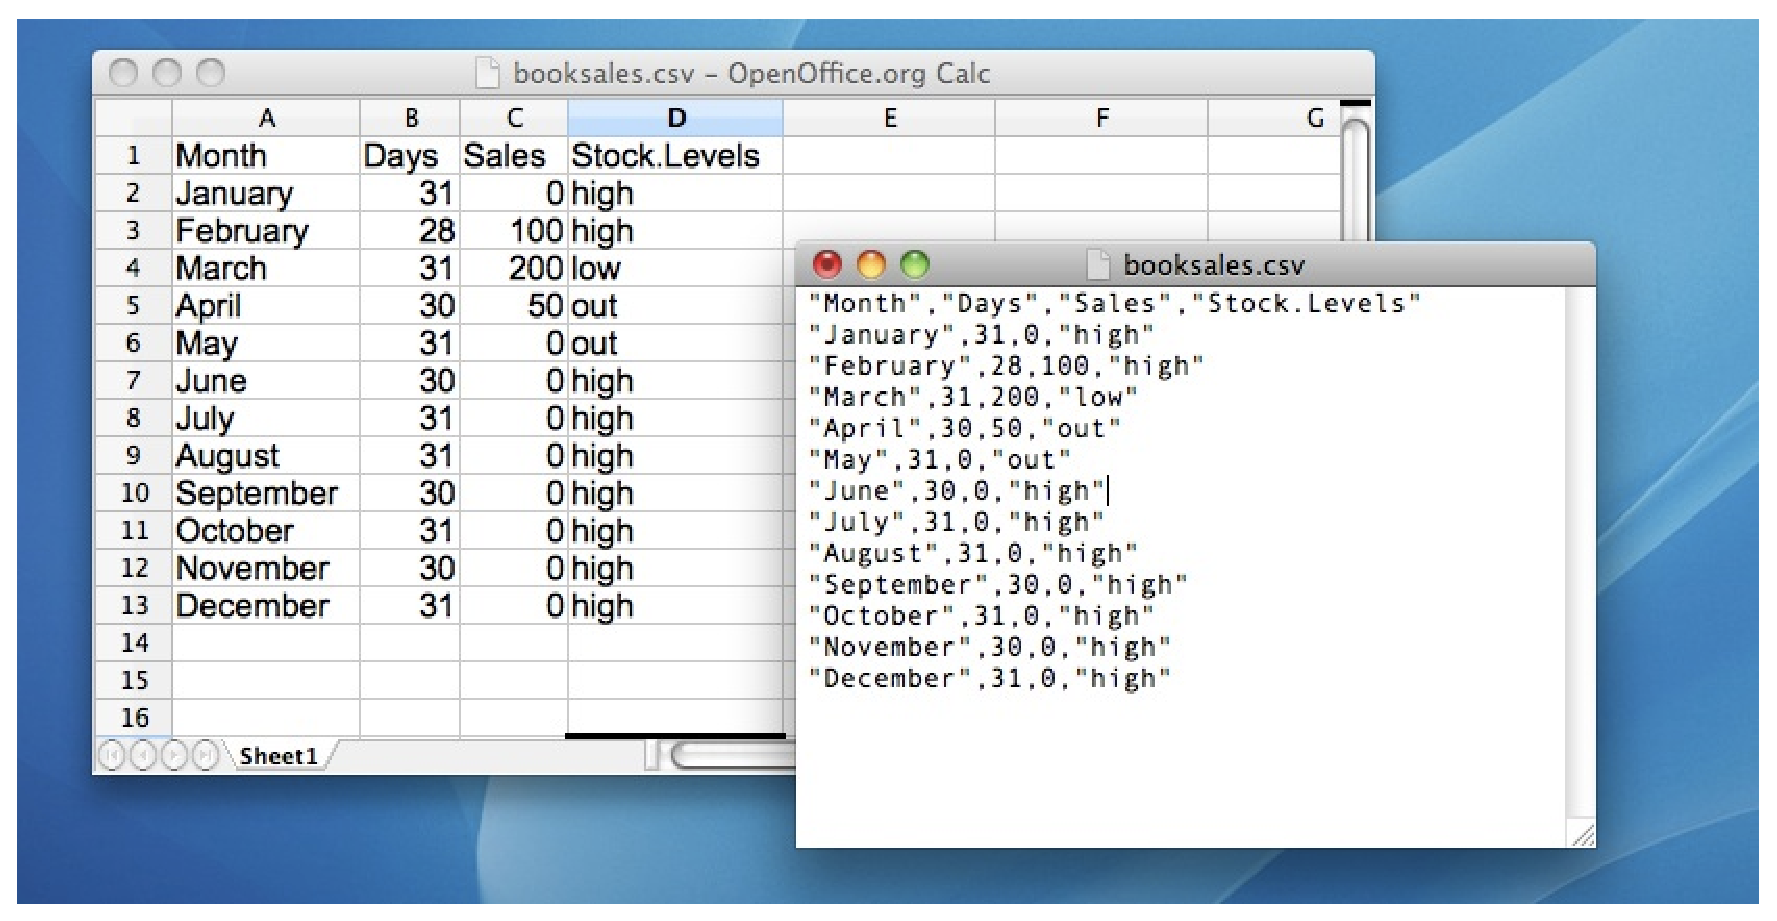
\epsfig{file = ../img/mechanics/booksalescsv.eps, clip=true,width = 14cm}
\caption{The \filename{booksales.csv} data file. On the left, I've opened the file in using a spreadsheet program (OpenOffice), which shows that the file is basically a table. On the right, the same file is open in a standard text editor (the TextEdit program on a Mac), which shows how the file is formatted. The entries in the table are wrapped in quote marks and separated by commas.}
\HR
\label{fig:booksalescsv}
\end{center}
\end{figure} 

If Rstudio were not available to you, the easiest way to open this file would be to use the \rtext{read.csv()} function.\FOOTNOTE{In a lot of books you'll see the \rtextsmall{read.table()} function used for this purpose instead of \rtextsmall{read.csv()}. They're more or less identical functions, with the same arguments and everything. They differ only in the default values.} This function is pretty flexible, and I'll talk a lot more about it's capabilities in Section~\ref{sec:importing} for more details, but for now there's only two arguments to the function that I'll mention:
\begin{itemize}
\item \rtext{file}. This should be a character string that specifies a path to the file that needs to be loaded. You can use an absolute path or a relative path to do so.
\item \rtext{header}. This is a logical value indicating whether or not the first row of the file contains variable names. The default value is \rtext{TRUE}. 
\end{itemize}
Therefore, to import the CSV file, the command I need is:
\begin{rblock1}
> @usr{books <- read.csv( file = "booksales.csv" )}
\end{rblock1}
There are two very important points to notice here. Firstly, notice that I {\it didn't} try to use the \rtext{load()} function, because that function is only meant to be used for \filename{.Rdata} files. If you try to use \rtext{load()} on other types of data, you get an error. Secondly, notice that when I imported the CSV file I assigned the result to a variable, which I imaginatively called \rtext{books}.\FOOTNOTE{Note that I didn't to this in my earlier example when loading the \filename{.Rdata} file. There's a reason for this. The idea behind an \filename{.Rdata} file is that it stores a whole workspace. So, if you had the ability to look inside the file yourself you'd see that the data file keeps track of all the variables and their names. So when you \rtextsmall{load()} the file, \R\ restores all those original names. CSV files are treated differently: as far as \R\ is concerned, the CSV only stores {\it one} variable, but that variable is big table. So when you import that table into the workspace, \R\ expects {\it you} to give it a name.} Let's have a look at what we've got:
\begin{rblock1}
> @usr{print( books )}
       Month Days Sales Stock.Levels
1    January   31     0         high
2   February   28   100         high
3      March   31   200          low
4      April   30    50          out
5        May   31     0          out
6       June   30     0         high
7       July   31     0         high
8     August   31     0         high
9  September   30     0         high
10   October   31     0         high
11  November   30     0         high
12  December   31     0         high
\end{rblock1}
Clearly, it's worked, but the format of this output is a bit unfamiliar. We haven't seen anything like this before. What you're looking at is a {\it data frame}, which is a very important kind of variable in \R, and one I'll discuss in Section~\ref{sec:dataframes}. For now, let's just be happy that we imported the data and that it looks about right.


\SUBSECTION{Importing data from CSV files using Rstudio}

Yet again, it's easier in Rstudio. In the environment panel in Rstudio you should see a button called ``Import Dataset''. Click on that, and it will give you a couple of options: select the ``From Text File...'' option, and it will open up a very familiar dialog box asking you to select a file: if you're on a Mac, it'll look like the usual Finder window that you use to choose a file; on Windows it looks like an Explorer window. An example of what it looks like on a Mac is shown in Figure~\ref{fig:fileopen}. I'm assuming that you're familiar with your own computer, so you should have no problem finding the CSV file that you want to import! Find the one you want, then click on the ``Open'' button. When you do this, you'll see a window that looks like the one in Figure~\ref{fig:import}.

\begin{figure}[t]
\begin{center}
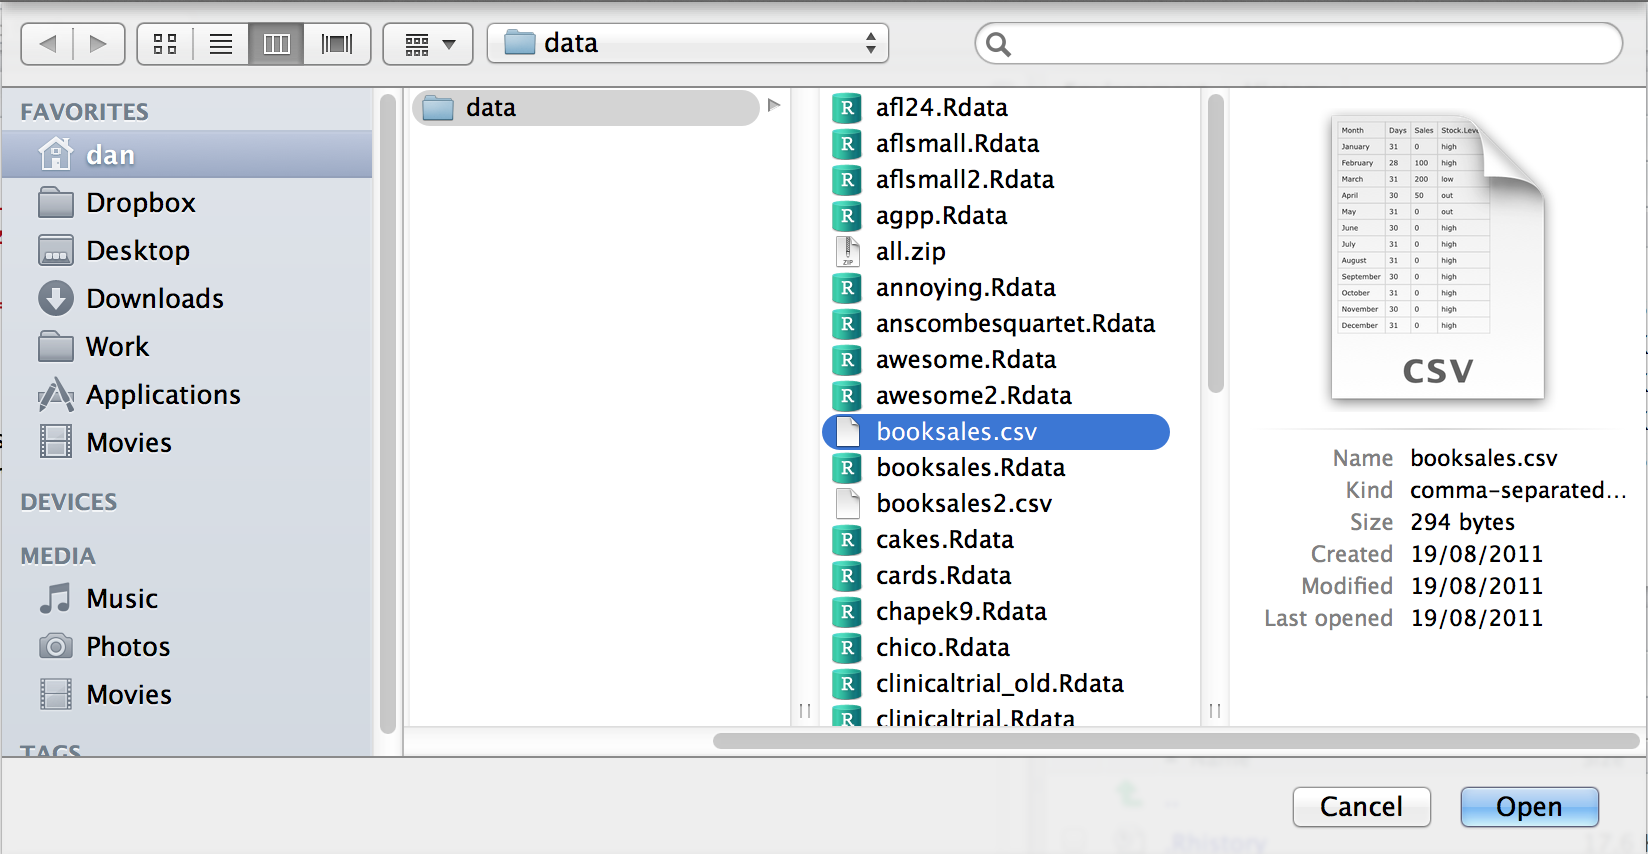
\epsfig{file = ../img/mechanics/openscreen.eps,clip=true, width = 14cm}
\caption{A dialog box on a Mac asking you to select the CSV file \R\ should try to import. Mac users will recognise this immediately: it's the usual way in which a Mac asks you to find a file. Windows users won't see this: they'll see the usual explorer window that Windows always gives you when it wants you to select a file.}
\HR
\label{fig:fileopen}
\end{center}
\end{figure} 


\begin{figure}[t]
\begin{center}
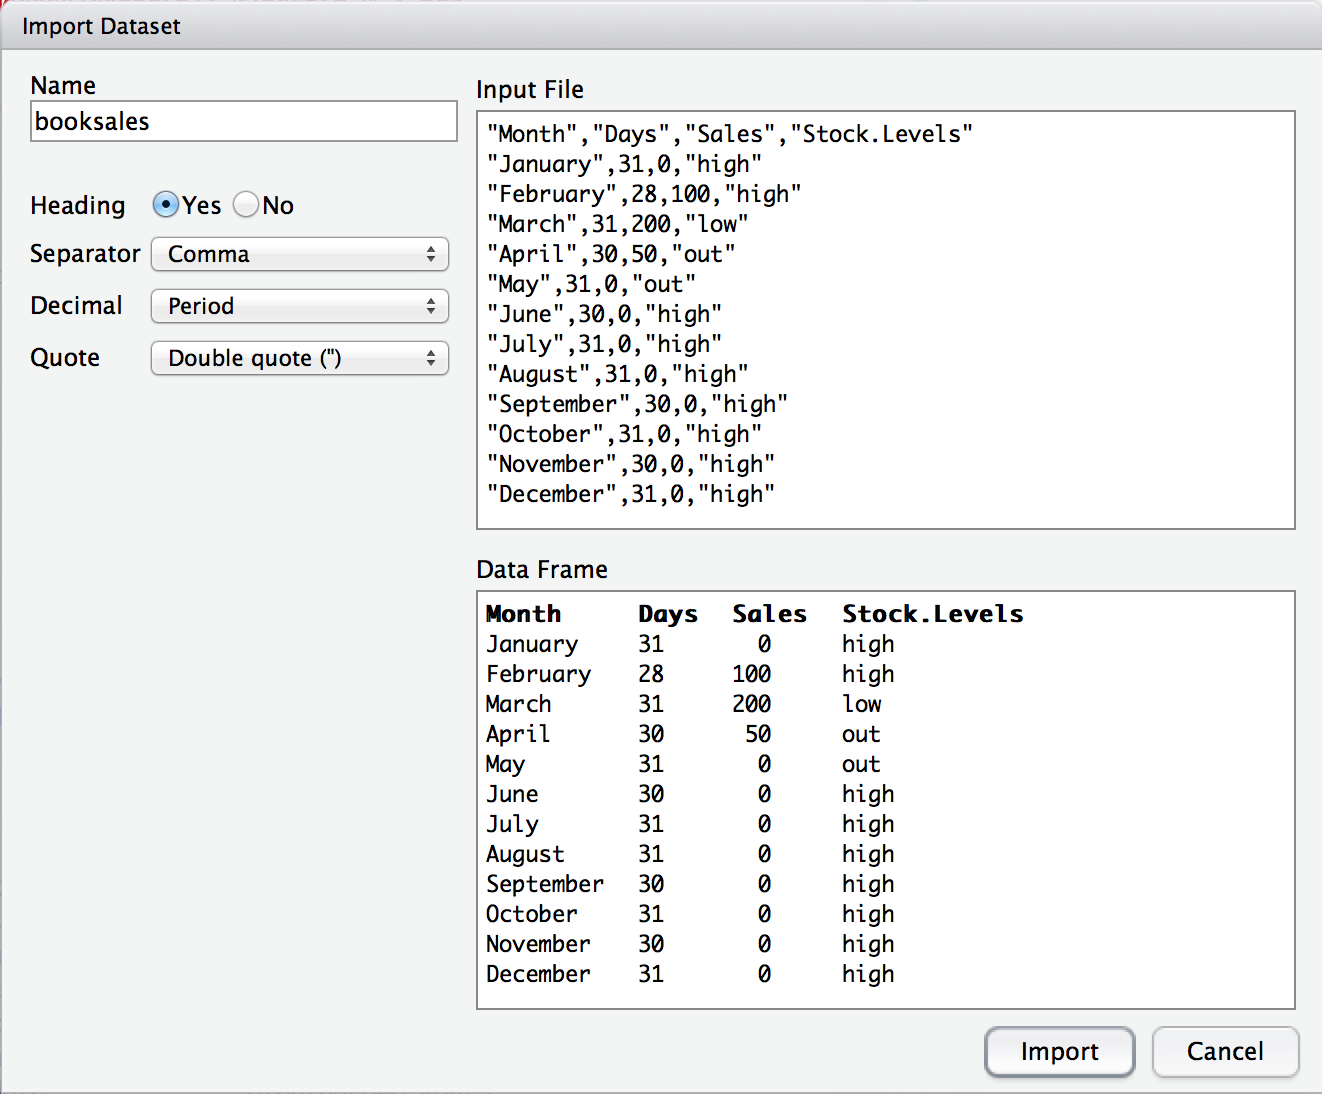
\epsfig{file = ../img/mechanics/import.eps,clip=true, width = 14cm}
\caption{The Rstudio window for importing a CSV file into \R.}
\HR
\label{fig:import}
\end{center}
\end{figure} 

The import data set window is relatively straightforward to understand. In the top left corner, you need to type the name of the variable you \R\ to create. By default, that will be the same as the file name: our file is called \texttt{booksales.csv}, so Rstudio suggests the name \rtext{booksales}. If you're happy with that, leave it alone. If not, type something else. Immediately below this are a few things that you can tweak to make sure that the data gets imported correctly: 

\begin{itemize}
\item Heading. Does the first row of the file contain raw data, or does it contain headings for each variable? The \texttt{booksales.csv} file has a header at the top, so I selected ``yes''.
\item Separator. What character is used to separate different entries? In most CSV files this will be a comma (it is ``comma separated'' after all). But you can change this if your file is different. 
\item Decimal. What character is used to specify the decimal point? In English speaking countries, this is almost always a period (i.e., \texttt{.}). That's not universally true: many European countries use a comma. So you can change that if you need to.
\item Quote. What character is used to denote a block of text? That's usually going to be a double quote mark. It is for the \texttt{booksales.csv} file, so that's what I selected.
\end{itemize}
The nice thing about the Rstudio window is that it shows you the raw data file at the top of the window, and it shows you a preview of the data at the bottom. If the data at the bottom doesn't look right, try changing some of the settings on the left hand side. Once you're happy, click ``Import''. When you do, two commands appear in the \R\ console:
\begin{rblock1}
> @usr{booksales <- read.csv("~/Rbook/data/booksales.csv")}
> @usr{View(booksales)}
\end{rblock1}
The first of these commands is the one that loads the data. The second one will display a pretty table showing the data in Rstudio. 


\SUBSECTION{Saving a workspace file using \R\label{sec:save}}

Not surprisingly, saving data is very similar to loading data. Although Rstudio provides a simple way to save files (see below), it's worth understanding the actual commands involved. There are two commands you can use to do this, \rtext{save()} and \rtext{save.image()}. If you're happy to save {\it all} of the variables in your workspace into the data file, then you should use \rtext{save.image()}. And if you're happy for \R\ to save the file into the current working directory, all you have to do is this:
\begin{rblock1}
> @usr{save.image( file = "myfile.Rdata" )}
\end{rblock1}
Since \rtext{file} is the first argument, you can shorten this to \rtext{save.image("myfile.Rdata")}; and if you want to save to a different directory, then (as always) you need to be more explicit about specifying the path to the file, just as we discussed in Section~\ref{sec:navigation}. Suppose, however, I have several variables in my workspace, and I only want to save some of them. For instance, I might have this as my workspace:
\begin{rblock1}
> @usr{who()}
   -- Name --   -- Class --   -- Size --
   data         data.frame    3 x 2     
   handy        character     1         
   junk         numeric       1        
\end{rblock1}
I want to save \rtext{data} and \rtext{handy}, but not \rtext{junk}. But I don't want to delete \rtext{junk} right now, because I want to use it for something else later on. This is where the \rtext{save()} function is useful, since it lets me indicate exactly which variables I want to save. Here is one way I can use the \rtext{save} function to solve my problem:
\begin{rblock1}
> @usr{save(data, handy, file = "myfile.Rdata")}
\end{rblock1}
Importantly, you {\it must} specify the name of the \rtext{file} argument. The reason is that if you don't do so, \R\ will think that \rtext{"myfile.Rdata"} is actually a {\it variable} that you want to save, and you'll get an error message. Finally, I should mention a second way to specify which variables the \rtext{save()} function should save, which is to use the \rtext{list} argument. You do so like this:
\begin{rblock1}
> @usr{save.me <- c("data", "handy")}   # the variables to be saved
> @usr{save( file = "booksales2.Rdata", list = save.me )}   # the command to save them
\end{rblock1}

\SUBSECTION{Saving a workspace file using Rstudio\label{sec:save1}}

Rstudio allows you to save the workspace pretty easily. In the environment panel (Figures~\ref{fig:workspace} and \ref{fig:workspace2}) you can see the ``save'' button. There's no text, but it's the same icon that gets used on every computer everywhere: it's the one that looks like a floppy disk. You know, those things that haven't been used in about 20 years. Alternatively, go to the ``Session'' menu and click on the ``Save Workspace As...'' option.\FOOTNOTE{A word of warning: what you \underline{don't} want to do is use the ``File'' menu. If you look in the ``File'' menu you will see ``Save'' and ``Save As...'' options, but they don't save the workspace. Those options are used for dealing with {\it scripts}, and so they'll produce \rtext{.R} files. We won't get to those until Chapter~\ref{ch:scripting}.} This will bring up the standard ``save'' dialog box for your operating system (e.g., on a Mac it'll look a little bit like the loading dialog box in Figure~\ref{fig:fileopen}). Type in the name of the file that you want to save it to, and all the variables in your workspace will be saved to disk. You'll see an \R\ command like this one
\begin{rblock1}
> @usr{save.image("~/Desktop/Untitled.RData")}
\end{rblock1}
Pretty straightforward, really.



\SUBSECTION{Other things you might want to save}

Until now, we've talked mostly about loading and saving {\it data}. Other things you might want to save include:

\begin{itemize}

\item {\it The output}. Sometimes you might also want to keep a copy of all your interactions with \R, including everything that you typed in and everything that \R\ did in response. There are some functions that you can use to get \R\ to write its output to a file rather than to print onscreen (e.g., \rtext{sink()}), but to be honest, if you do want to save the \R\ output, the easiest thing to do is to use the mouse to select the relevant text in the \R\ console, go to the ``Edit'' menu in Rstudio and select ``Copy''. The output has now been copied to the clipboard. Now open up your favourite text editor or word processing software, and paste it. And you're done.  However, this will only save the contents of the console, not the plots you've drawn (assuming you've drawn some). We'll talk about saving images later on.


\item {\it A script}. While it is possible -- and sometimes handy -- to save the \R\ output as a method for keeping a copy of your statistical analyses, another option that people use a lot (especially when you move beyond simple ``toy'' analyses) is to write {\it scripts}. A script is a text file in which you write out all the commands that you want \R\ to run. You can write your script using whatever software you like. In real world data analysis writing scripts is a key skill -- and as you become familiar with \R\ you'll probably find that most of what you do involves scripting rather than typing commands at the \R\ prompt. However, you won't need to do much scripting initially, so we'll leave that until Chapter~\ref{ch:scripting}.

\end{itemize}




\section{Useful things to know about variables~\label{sec:useful}}

In Chapter~\ref{ch:introR} I talked a lot about variables, how they're assigned and some of the things you can do with them, but there's a lot of additional complexities. That's not a surprise of course. However, some of those issues are worth drawing your attention to now. So that's the goal of this section; to cover a few extra topics. As a consequence, this section is basically a bunch of things that I want to briefly mention, but don't really fit in anywhere else. In short, I'll talk about several different issues in this section, which are only loosely connected to one another.



\SUBSECTION{Special values\label{sec:specials}}

The first thing I want to mention are some of the ``special'' values that you might see \R\ produce. Most likely you'll see them in situations where you were expecting a number, but there are quite a few other ways you can encounter them. These values are \rtext{Inf}, \rtext{NaN}, \rtext{NA} and \rtext{NULL}. These values can crop up in various different places, and so it's important to understand what they mean. 

\begin{itemize}
%\SUBSECTION{Infinity, \rtext{Inf}}

\item \underline{\it Infinity} (\rtext{Inf}). The easiest of the special values to explain is \rtext{Inf}, since it corresponds to a value that is infinitely large. You can also have \rtext{-Inf}. The easiest way to get \rtext{Inf} is to divide a positive number by 0:
\begin{rblock1}
> @usr{1 / 0}
[1] Inf
\end{rblock1}
In most real world data analysis situations, if you're ending up with infinite numbers in your data, then something has gone awry. Hopefully you'll never have to see them.
\vspace*{6pt}
%\SUBSECTION{Not a number, \rtext{NaN}}

\item \underline{\it Not a Number} (\rtext{NaN}). The special value of \rtext{NaN} is short for ``not a number'', and it's basically a reserved keyword that means ``there isn't a mathematically defined number for this''. If you can remember your high school maths, remember that it is conventional to say that $0/0$ doesn't have a proper answer: mathematicians would say that $0/0$ is {\it undefined}. \R\ says that it's not a number:
\begin{rblock1}
> @usr{0 / 0}
[1] NaN
\end{rblock1}
Nevertheless, it's still treated as a ``numeric'' value. To oversimplify, \rtext{NaN} corresponds to cases where you asked a proper numerical question that genuinely has {\it no meaningful answer}. 
\vspace*{6pt}


%\SUBSECTION{Not available, \rtext{NA}}
\item \underline{\it Not available} (\rtext{NA}). 
\rtext{NA} indicates that the value that is ``supposed'' to be stored here is missing. To understand what this means, it helps to recognise that the \rtext{NA} value is something that you're most likely to see when analysing data from real world experiments. Sometimes you get equipment failures, or you lose some of the data, or whatever. The point is that some of the information that you were ``expecting'' to get from your study is just plain missing. Note the difference between \rtext{NA} and \rtext{NaN}. For \rtext{NaN}, we really do know what's supposed to be stored; it's just that it happens to correspond to something like $0/0$ that doesn't make any sense at all. In contrast, \rtext{NA} indicates that we actually don't know what was supposed to be there. The information is {\it missing}.
\vspace*{6pt}

%\SUBSECTION{No value, \rtext{NULL}}
\item \underline{\it No value} (\rtext{NULL}).
The \rtext{NULL} value takes this ``absence'' concept even further. It basically asserts that the variable genuinely has no value whatsoever. This is quite different to both \rtext{NaN} and \rtext{NA}. For \rtext{NaN} we actually know what the value is, because it's something insane like $0/0$. For \rtext{NA}, we believe that there is supposed to be a value ``out there'', but a dog ate our homework and so we don't quite know what it is. But for \rtext{NULL} we strongly believe that there is {\it no value at all}.  

\end{itemize}



\SUBSECTION{Assigning names to vector elements~\label{sec:names}}

One thing that is sometimes a little unsatisfying about the way that \R\ prints out a vector is that the elements come out unlabelled. Here's what I mean. Suppose I've got data reporting the quarterly profits for some company. If I just create a no-frills vector, I have to rely on memory to know which element corresponds to which event. That is:
\begin{rblock1}
> @usr{profit <- c( 3.1, 0.1, -1.4, 1.1 )}
> @usr{profit}
[1]  3.1  0.1 -1.4  1.1
\end{rblock1}
You can probably guess that the first element corresponds to the first quarter, the second element to the second quarter, and so on, but that's only because I've told you the back story and because this happens to be a very simple example. In general, it can be quite difficult. This is where it can be helpful to assign \rtext{names} to each of the elements. Here's how you do it:
\begin{rblock1}
> @usr{names(profit) <- c("Q1","Q2","Q3","Q4")}
> @usr{profit}
  Q1   Q2   Q3   Q4 
 3.1  0.1 -1.4  1.1 
\end{rblock1}
This is a slightly odd looking command, admittedly, but it's not too difficult to follow. All we're doing is assigning a vector of labels (character strings) to \rtext{names(profit)}. You can always delete the names again by using the command \rtext{names(profit) <- NULL}. It's also worth noting that you don't have to do this as a two stage process. You can get the same result with this command:
\begin{rblock1}
> @usr{profit <- c( "Q1" = 3.1, "Q2" = 0.1, "Q3" = -1.4, "Q4" = 1.1 )}
> @usr{profit}
  Q1   Q2   Q3   Q4 
 3.1  0.1 -1.4  1.1 
 \end{rblock1}
The important things to notice are that (a) this does make things much easier to read, but (b) the names at the top aren't the ``real'' data. The {\it value} of \rtext{profit[1]} is still \rtext{3.1}; all I've done is added a {\it name} to \rtext{profit[1]} as well. Nevertheless, names aren't purely cosmetic, since \R\ allows you to pull out particular elements of the vector by referring to their names:
\begin{rblock1}
> @usr{profit["Q1"]}
 Q1 
3.1  
\end{rblock1}
And if I ever need to pull out the names themselves, then I just type \rtext{names(profit)}. 

\SUBSECTION{Variable classes}

As we've seen, \R\ allows you to store different kinds of data. In particular, the variables we've defined so far have either been character data (text), numeric data, or logical data.\FOOTNOTE{Or functions. But let's ignore functions for the moment.} It's important that we remember what kind of information each variable stores (and even more important that \R\ remembers) since different kinds of variables allow you to do different things to them. For instance, if your variables have numerical information in them, then it's okay to multiply them together:
\begin{rblock1}
> @usr{x <- 5}   # x is numeric
> @usr{y <- 4}   # y is numeric
> @usr{x * y}    
[1] 20
\end{rblock1}
But if they contain character data, multiplication makes no sense whatsoever, and \R\ will complain if you try to do it:
\begin{rblock1}
> @usr{x <- "apples"}   # x is character
> @usr{y <- "oranges"}  # y is character
> @usr{x * y}           
Error in x * y : non-numeric argument to binary operator
\end{rblock1}
Even \R\ is smart enough to know you can't multiply \rtext{"apples"} by \rtext{"oranges"}. It knows this because the quote marks are indicators that the variable is supposed to be treated as text, not as a number. 

This is quite useful, but notice that it means that \R\ makes a big distinction between \rtext{5} and \rtext{"5"}. Without quote marks, \R\ treats \rtext{5} as the number five, and will allow you to do calculations with it. With the quote marks, \R\ treats \rtext{"5"} as the textual character five, and doesn't recognise it as a number any more than it recognises \rtext{"p"} or \rtext{"five"} as numbers.  As a consequence, there's a big difference between typing \rtext{x <- 5} and typing \rtext{x <- "5"}. In the former, we're storing the number \rtext{5}; in the latter, we're storing the character \rtext{"5"}. Thus, if we try to do multiplication with the character versions, \R\ gets stroppy:
\begin{rblock1}
> @usr{x <- "5"}   # x is character
> @usr{y <- "4"}   # y is character
> @usr{x * y}     
Error in x * y : non-numeric argument to binary operator
\end{rblock1}

Okay, let's suppose that I've forgotten what kind of data I stored in the variable \rtext{x} (which happens depressingly often). \R\ provides a function that will let us find out. Or, more precisely, it provides {\it three} functions: \rtext{class()}, \rtext{mode()} and \rtext{typeof()}. Why the heck does it provide three functions, you might be wondering? Basically, because \R\ actually keeps track of three different kinds of information about a variable:
\begin{enumerate}
\item The \keyterm{class} of a variable is a ``high level'' classification, and it captures psychologically (or statistically) meaningful distinctions. For instance \rtext{"2011-09-12"} and \rtext{"my birthday"} are both text strings, but there's an important difference between the two: one of them is a date. So it would be nice if we could get \R\ to recognise that \rtext{"2011-09-12"} is a date, and allow us to do things like add or subtract from it. The class of a variable is what \R\ uses to keep track of things like that. Because the class of a variable is critical for determining what \R\ can or can't do with it, the \rtext{class()} function is very handy.
\item The \keyterm{mode} of a variable refers to the format of the information that the variable stores. It tells you whether \R\ has stored text data or numeric data, for instance, which is kind of useful, but it only makes these ``simple'' distinctions. It can be useful to know about, but it's not the main thing we care about. So I'm not going to use the \rtext{mode()} function very much.\FOOTNOTE{Actually, I don't think I {\it ever} use this in practice. I don't know why I bother to talk about it in the book anymore.} 
\item The \keyterm{type} of a variable is a very low level classification. We won't use it in this book, but (for those of you that care about these details) this is where you can see the distinction between integer data, double precision numeric, etc. Almost none of you actually will care about this, so I'm not even going to bother demonstrating the \rtext{typeof()} function.
\end{enumerate}

\noindent
For purposes, it's the \rtext{class()} of the variable that we care most about. Later on, I'll talk a bit about how you can convince \R\ to ``coerce'' a variable to change from one class to another (Section~\ref{sec:coercion}). That's a useful skill for real world data analysis, but it's not something that we need right now. In the meantime, the following examples illustrate the use of the \rtext{class()} function:
\begin{rblock1}
> @usr{x <- "hello world"}     # x is text
> @usr{class(x)}
[1] "character"

> @usr{x <- TRUE}     # x is logical 
> @usr{class(x)}
[1] "logical"

> @usr{x <- 100}     # x is a number
> @usr{class(x)}
[1] "numeric"
\end{rblock1}
Exciting, no?





\section{Factors\label{sec:factors}}


Okay, it's time to start introducing some of the data types that are somewhat more specific to statistics. If you remember back to Chapter~\ref{ch:studydesign}, when we assign numbers to possible outcomes, these numbers can mean quite different things depending on what kind of variable we are attempting to measure. In particular, we commonly make the distinction between {\it nominal}, {\it ordinal}, {\it interval} and {\it ratio} scale data. How do we capture this distinction in \R? Currently, we only seem to have a single numeric data type. That's probably not going to be enough, is it?

A little thought suggests that the numeric variable class in \R\ is perfectly suited for capturing ratio scale data. For instance, if I were to measure response time (RT) for five different events, I could store the data in \R\ like this:
\begin{rblock1}
> @usr{RT <- c(342, 401, 590, 391, 554)}
\end{rblock1}
where the data here are measured in milliseconds, as is conventional in the psychological literature. It's perfectly sensible to talk about ``twice the response time'', $2 \times \mbox{RT}$, or the ``response time plus 1 second'', $\mbox{RT} + 1000$, and so both of the following are perfectly reasonable things for \R\ to do:
\begin{rblock1}
> @usr{2 * RT}
[1]  684  802 1180  782 1108
> @usr{RT + 1000}
[1] 1342 1401 1590 1391 1554
\end{rblock1} 
And to a lesser extent, the ``numeric'' class is okay for interval scale data, as long as we remember that multiplication and division aren't terribly interesting for these sorts of variables. That is, if my IQ score is 110 and yours is 120, it's perfectly okay to say that you're 10 IQ points smarter than me\FOOTNOTE{Taking all the usual caveats that attach to IQ measurement as a given, of course.}, but it's not okay to say that I'm only 92\% as smart as you are, because intelligence doesn't have a natural zero.\FOOTNOTE{Or, more precisely, we don't know how to measure it. Arguably, a rock has zero intelligence. But it doesn't make sense to say that the IQ of a rock is 0 in the same way that we can say that the average human has an IQ of 100. And without knowing what the IQ value is that corresponds to a literal absence of any capacity to think, reason or learn, then we really can't multiply or divide IQ scores and expect a meaningful answer.} We might even be willing to tolerate the use of numeric variables to represent ordinal scale variables, such as those that you typically get when you ask people to rank order items (e.g., like we do in Australian elections), though as we will see \R\ actually has a built in tool for representing ordinal data (see Section~\ref{sec:orderedfactors}) However, when it comes to nominal scale data, it becomes completely unacceptable, because almost all of the ``usual'' rules for what you're allowed to do with numbers don't apply to nominal scale data. It is for this reason that \R\ has \keyterm{factors}. 



\SUBSECTION{Introducing factors}

Suppose, I was doing a study in which people could belong to one of three different treatment conditions. Each group of people were asked to complete the same task, but each group received different instructions. Not surprisingly, I might want to have a variable that keeps track of what group people were in. So I could type in something like this
\begin{rblock1}
> @usr{group <- c(1,1,1,2,2,2,3,3,3)}
\end{rblock1}
so that \rtext{group[i]} contains the group membership of the \rtext{i}-th person in my study. Clearly, this is numeric data, but equally obviously this is a nominal scale variable. There's no sense in which ``group 1'' plus ``group 2'' equals ``group 3'', but nevertheless if I try to do that, \R\ won't stop me because it doesn't know any better:
\begin{rblock1}
> @usr{group + 2}
 [1] 3 3 3 4 4 4 5 5 5 
\end{rblock1}
Apparently \R\ seems to think that it's allowed to invent ``group 4'' and ``group 5'', even though they didn't actually exist. Unfortunately, \R\ is too stupid to know any better: it thinks that \rtext{3} is an ordinary number in this context, so it sees no problem in calculating \rtext{3 + 2}. But since {\it we're} not that stupid, we'd like to stop \R\ from doing this. We can do so by instructing \R\ to treat \rtext{group} as a factor.  This is easy to do using the \rtext{as.factor()} function.\FOOTNOTE{Once again, this is an example of {\it coercing} a variable from one class to another. I'll talk about coercion in more detail in Section~\ref{sec:coercion}.} 
\begin{rblock1}
> @usr{group <- as.factor(group)}
> @usr{group}
 [1] 1 1 1 2 2 2 3 3 3 
 Levels: 1 2 3
\end{rblock1}
It looks more or less the same as before (though it's not immediately obvious what all that \rtextoutput{Levels} rubbish is about), but if we ask \R\ to tell us what the class of the \rtext{group} variable is now, it's clear that it has done what we asked:
\begin{rblock1}
> @usr{class(group)}
[1] "factor"
\end{rblock1}
Neat. Better yet, now that I've converted \rtext{group} to a factor, look what happens when I try to add 2 to it:
\begin{rblock1}
> @usr{group + 2}
[1] NA NA NA NA NA NA NA NA NA
Warning message:
In Ops.factor(group, 2) : + not meaningful for factors
\end{rblock1}
This time even \R\ is smart enough to know that I'm being an idiot, so it tells me off and then produces a vector of missing values. % (i.e., \rtextoutput{NA}: see Section~\ref{sec:specials}).


\SUBSECTION{Labelling the factor levels}

I have a confession to make. My memory is not infinite in capacity; and it seems to be getting worse as I get older. So it kind of annoys me when I get data sets where there's a nominal scale variable called \rtext{gender}, with two levels corresponding to males and females. But when I go to print out the variable I get something like this:
\begin{rblock1}
> @usr{gender}
[1] 1 1 1 1 1 2 2 2 2
Levels: 1 2
\end{rblock1}
Okaaaay. That's not helpful at all, and it makes me very sad. Which number corresponds to the males and which one corresponds to the females? Wouldn't it be nice if \R\ could actually keep track of this? It's way too hard to remember which number corresponds to which gender. And besides, the problem that this causes is much more serious than a single sad nerd... because \R\ has no way of knowing that the \rtext{1}s in the \rtext{group} variable are a very different kind of thing to the \rtext{1}s in the \rtext{gender} variable. So if I try to ask which elements of the \rtext{group} variable are equal to the corresponding elements in \rtext{gender}, \R\ thinks this is totally kosher, and gives me this:
\begin{rblock1}
> @usr{group == gender}
[1]  TRUE  TRUE  TRUE FALSE FALSE  TRUE FALSE FALSE FALSE
\end{rblock1}
Well, that's ... especially stupid.\FOOTNOTE{Some users might wonder why \R\ even allows the \rtextsmall{==} operator for factors. The reason is that sometimes you really do have different factors that have the same levels. For instance, if I was analysing data associated with football games, I might have a factor called \rtextsmall{home.team}, and another factor called \rtextsmall{winning.team}. In that situation I really should be able to ask if \rtextsmall{home.team == winning.team}.}  The problem here is that \R\ is very literal minded. Even though you've declared both \rtext{group} and \rtext{gender} to be factors, it still assumes that a \rtext{1} is a \rtext{1} no matter which variable it appears in. 

To fix both of these problems (my memory problem, and \R's infuriating literal interpretations), what we need to do is assign meaningful labels to the different {\it levels} of each factor. We can do that like this:
\begin{rblock1}
> @usr{levels(group) <- c("group 1", "group 2", "group 3")}
> @usr{print(group)}
[1] group 1 group 1 group 1 group 2 group 2 group 2 group 3 group 3 group 3
Levels: group 1 group 2 group 3
> 
> @usr{levels(gender) <- c("male", "female")}
> @usr{print(gender)}
[1] male   male   male   male   male   female female female female
Levels: male female
\end{rblock1}
That's much easier on the eye, and better yet, \R\ is smart enough to know that \rtext{"female"} is not equal to \rtext{"group 2"}, so now when I try to ask which group memberships are ``equal to'' the gender of the corresponding person, 
\begin{rblock1}
> @usr{group == gender}
Error in Ops.factor(group, gender) : level sets of factors are different
\end{rblock1}
\R\ correctly tells me that I'm an idiot.


\SUBSECTION{Moving on...}

Factors are very useful things, and we'll use them a lot in this book: they're {\it the} main way to represent a nominal scale variable. And there are lots of nominal scale variables out there. I'll talk more about factors in \ref{sec:orderedfactors}, but for now you know enough to be able to get started.




\section{Data frames\label{sec:dataframes}}

It's now time to go back and deal with the somewhat confusing thing that happened in Section~\ref{sec:loadingcsv} when we tried to open up a CSV file. Apparently we succeeded in loading the data, but it came to us in a very odd looking format. At the time, I told you that this was a \keyterm{data frame}. Now I'd better explain what that means.



\SUBSECTION{Introducing data frames}

In order to understand why \R\ has created this funny thing called a data frame, it helps to try to see what problem it solves. So let's go back to the little scenario that I used when introducing factors in Section~\ref{sec:factors}. In that section I recorded the \rtext{group} and \rtext{gender} for all 9 participants in my study. Let's also suppose I recorded their ages and their \rtext{score} on ``Dan's Terribly Exciting Psychological Test'':
\begin{rblock1}
> @usr{age <- c(17, 19, 21, 37, 18, 19, 47, 18, 19)}
> @usr{score <- c(12, 10, 11, 15, 16, 14, 25, 21, 29)}
\end{rblock1}
Assuming no other variables are in the workspace, if I type \rtext{who()} I get this:
\begin{rblock1}
> @usr{who()}
   -- Name --   -- Class --   -- Size --
   age          numeric       9         
   gender       factor        9         
   group        factor        9         
   score        numeric       9          
\end{rblock1}
So there are four variables in the workspace, \rtext{age}, \rtext{gender}, \rtext{group} and \rtext{score}. And it just so happens that all four of them are the same size (i.e., they're all vectors with 9 elements). Aaaand it just so happens that \rtext{age[1]} corresponds to the age of the first person, and \rtext{gender[1]} is the gender of that very same person, etc. In other words, you and I both know that all four of these variables correspond to the {\it same} data set, and all four of them are organised in exactly the same way. 

However, \R\ {\it doesn't} know this! As far as it's concerned, there's no reason why the \rtext{age} variable has to be the same length as the \rtext{gender} variable; and there's no particular reason to think that \rtext{age[1]} has any special relationship to \rtext{gender[1]} any more than it has a special relationship to \rtext{gender[4]}. In other words, when we store everything in separate variables like this, \R\ doesn't know anything about the relationships between things. It doesn't even really know that these variables actually refer to a proper data set. The data frame fixes this: if we store our variables inside a data frame, we're telling \R\ to treat these variables as a single, fairly coherent data set. 

To see how they do this, let's create one. So how do we create a data frame? One way we've already seen: if we import our data from a CSV file, \R\ will store it as a data frame. A second way is to create it directly from some existing variables using the \rtext{data.frame()} function. All you have to do is type a list of variables that you want to include in the data frame. The output of a \rtext{data.frame()} command is, well, a data frame. So, if I want to store all four variables from my experiment in a data frame called \rtext{expt} I can do so like this:
\begin{rblock1}
> @usr{expt <- data.frame ( age, gender, group, score )} 
> @usr{expt} 
  age gender   group score
1  17   male group 1    12
2  19   male group 1    10
3  21   male group 1    11
4  37   male group 2    15
5  18   male group 2    16
6  19 female group 2    14
7  47 female group 3    25
8  18 female group 3    21
9  19 female group 3    29
\end{rblock1}
Note that \rtext{expt} is a completely self-contained variable. Once you've created it, it no longer depends on the original variables from which it was constructed. That is, if we make changes to the original \rtext{age} variable, it will {\it not} lead to any changes to the age data stored in \rtext{expt}. 



\SUBSECTION{Pulling out the contents of the data frame using \rtext{\$}}

At this point, our workspace contains only the one variable, a data frame called \rtext{expt}. But as we can see when we told \R\ to print the variable out, this data frame contains 4 variables, each of which has 9 observations. So how do we get this information out again? After all, there's no point in storing information if you don't use it, and there's no way to use information if you can't access it. So let's talk a bit about how to pull information out of a data frame. 

The first thing we might want to do is pull out one of our stored variables, let's say \rtext{score}. One thing you might try to do is ignore the fact that \rtext{score} is locked up inside the \rtext{expt} data frame. For instance, you might try to print it out like this:
\begin{rblock1}
> @usr{score}
Error: object 'score' not found
\end{rblock1}
This doesn't work, because \R\ doesn't go ``peeking'' inside the data frame unless you explicitly tell it to do so. There's actually a very good reason for this, which I'll explain in a moment, but for now let's just assume \R\ knows what it's doing. How do we tell \R\ to look inside the data frame? As is always the case with \R\ there are several ways. The simplest way is to use the \rtextverb#$# operator to extract the variable you're interested in, like this:
\begin{rblock1}
> @usr{expt$score}
[1] 12 10 11 15 16 14 25 21 29
\end{rblock1}



\SUBSECTION{Getting information about a data frame}

One problem that sometimes comes up in practice is that you forget what you called all your variables. Normally you might try to type \rtext{objects()} or \rtext{who()}, but neither of those commands will tell you what the names are for those variables inside a data frame! One way is to ask \R\ to tell you what the {\it names} of all the variables stored in the data frame are, which you can do using the \rtext{names()} function:
\begin{rblock1}
> @usr{names(expt)}
[1] "age"    "gender" "group"  "score" 
\end{rblock1}
An alternative method is to use the \rtext{who()} function, as long as you tell it to look at the variables inside data frames. If you set \rtext{expand = TRUE} then it will not only list the variables in the workspace, but it will ``expand'' any data frames that you've got in the workspace, so that you can see what they look like. That is:
\begin{rblock1}
> @usr{who(expand = TRUE)}
   -- Name --   -- Class --   -- Size --
   expt         data.frame    9 x 4     
    $age        numeric       9         
    $gender     factor        9         
    $group      factor        9         
    $score      numeric       9         
\end{rblock1}
or, since \rtext{expand} is the first argument in the \rtext{who()} function you can just type \rtext{who(TRUE)}. I'll do that a lot in this book.


\SUBSECTION{Looking for more on data frames?}

There's a lot more that can be said about data frames: they're fairly complicated beasts, and the longer you use \R\ the more important it is to make sure you really understand them. We'll talk a lot more about them in Chapter~\ref{ch:datahandling}.







\section{Lists~\label{sec:lists}}

The next kind of data I want to mention are \keyterm{lists}. Lists are an extremely fundamental data structure in \R, and as you start making the transition from a novice to a savvy \R\ user you will use lists all the time. I don't use lists very often in this book -- not directly -- but most of the advanced data structures in \R\ are built from lists (e.g., data frames are actually a specific type of list). Because lists are so important to how \R\ stores things, it's useful to have a basic understanding of them. Okay, so what is a list, exactly? Like data frames, lists are just ``collections of variables.'' However, unlike data frames -- which are basically supposed to look like a nice ``rectangular'' table of data -- there are no constraints on what kinds of variables we include, and no requirement that the variables have any particular relationship to one another. In order to understand what this actually {\it means}, the best thing to do is create a list, which we can do using the \rtext{list()} function. If I type this as my command:
\begin{rblock1}
> @usr{Dan <- list( age = 34,}
+ @usr{             nerd = TRUE,}
+ @usr{             parents = c("Joe","Liz") }
+ @usr{)}
\end{rblock1}
\R\ creates a new list variable called \rtext{Dan}, which is a bundle of three different variables: \rtext{age}, \rtext{nerd} and \rtext{parents}. Notice, that the \rtext{parents} variable is longer than the others. This is perfectly acceptable for a list, but it wouldn't be for a data frame. If we now print out the variable, you can see the way that \R\ stores the list:
\begin{rblock1}
> @usr{print( Dan )}
$age
[1] 34

$nerd
[1] TRUE

$parents
[1] "Joe" "Liz" 
\end{rblock1}
As you might have guessed from those \rtextverb#$# symbols everywhere, the variables are stored in exactly the same way that they are for a data frame (again, this is not surprising: data frames {\it are} a type of list). So you will (I hope) be entirely unsurprised and probably quite bored when I tell you that you can extract the variables from the list using the \rtextverb#$# operator, like so:
\begin{rblock1}
> @usr{Dan$nerd}
[1] TRUE
\end{rblock1}
If you need to add new entries to the list, the easiest way to do so is to again use \rtextverb#$#, as the following example illustrates. If I type a command like this
\begin{rblock1}
> @usr{Dan$children <- "Alex"}
\end{rblock1}
then \R\ creates a new entry to the end of the list called \rtext{children}, and assigns it a value of \rtext{"Alex"}. If I were now to \rtext{print()} this list out, you'd see a new entry at the bottom of the printout. Finally, it's actually possible for lists to contain other lists, so it's quite possible that I would end up using a command like \rtextverb#Dan$children$age# to find out how old my son is. Or I could try to remember it myself I suppose. 




\section{Formulas\label{sec:formulas}}
 
The last kind of variable that I want to introduce before finally being able to start talking about statistics is the \keyterm{formula}. Formulas were originally introduced into \R\ as a convenient way to specify a particular type of statistical model (see Chapter~\ref{ch:regression}) but they're such handy things that they've spread. Formulas are now used in a lot of different contexts, so it makes sense to introduce them early.

Stated simply, a formula object is a variable, but it's a special type of variable that specifies a relationship between other variables. A formula is specified using the ``tilde operator'' \rtextverb#~#. A very simple example of a formula is shown below:\FOOTNOTE{Note that, when I write out the formula, \R\ doesn't check to see if the \rtextsmall{out} and \rtextsmall{pred} variables actually exist: it's only later on when you try to use the formula for something that this happens.}
\begin{rblock1}
> @usr{formula1 <- out ~ pred}
> @usr{formula1}
out ~ pred
\end{rblock1}
The {\it precise} meaning of this formula depends on exactly what you want to do with it, but in broad terms it means ``the \rtext{out} (outcome) variable, analysed in terms of the \rtext{pred} (predictor) variable''. That said, although the simplest and most common form of a formula uses the  ``one variable on the left, one variable on the right'' format, there are others. For instance, the following examples are all reasonably common
\begin{rblock1}
> @usr{formula2 <-  out ~ pred1 + pred2}   # more than one variable on the right
> @usr{formula3 <-  out ~ pred1 * pred2}   # different relationship between predictors 
> @usr{formula4 <-  ~ var1 + var2}         # a 'one-sided' formula
\end{rblock1}
and there are many more variants besides. Formulas are pretty flexible things, and so different functions will make use of different formats, depending on what the function is intended to do.


\section{Generic functions~\label{sec:generics}}

There's one really important thing that I omitted when I discussed functions earlier on in Section~\ref{sec:usingfunctions}, and that's the concept of a \keyterm{generic function}. The two most notable examples that you'll see in the next few chapters are \rtext{summary()} and \rtext{plot()}, although you've already seen an example of one working behind the scenes, and that's the \rtext{print()} function. The thing that makes generics different from the other functions is that their behaviour changes, often quite dramatically, depending on the \rtext{class()} of the input you give it. The easiest way to explain the concept is with an example. With that in mind, lets take a closer look at what the \rtext{print()} function actually does. I'll do this by creating a formula, and printing it out in a few different ways. First, let's stick with what we know:
\begin{rblock1}
> @usr{my.formula <- blah ~ blah.blah }   # create a variable of class "formula"
> @usr{print( my.formula )}               # print it out using the generic print() function
blah ~ blah.blah
\end{rblock1}
So far, there's nothing very surprising here. But there's actually a lot going on behind the scenes here. When I type \rtext{print( my.formula )}, what actually happens is the \rtext{print()} function checks the class of the \rtext{my.formula} variable. When the function discovers that the variable it's been given is a formula, it goes looking for a function called \rtext{print.formula()}, and then delegates the whole business of printing out the variable to the \rtext{print.formula()} function.\FOOTNOTE{For readers with a programming background: what I'm describing is the very basics of how S3 methods work. However, you should be aware that \R\ has two entirely distinct systems for doing object oriented programming, known as S3 and S4. Of the two, S3 is simpler and more informal, whereas S4 supports all the stuff that you might expect of a fully object oriented language. Most of the generics we'll run into in this book use the S3 system, which is convenient for me because I'm still trying to figure out S4. } For what it's worth, the name for a ``dedicated'' function like \rtext{print.formula()} that exists only to be a special case of a generic function like \rtext{print()} is a \keyterm{method}, and the name for the process in which the generic function passes off all the hard work onto a method is called \keyterm{method dispatch}. You won't need to understand the details at all for this book, but you do need to know the gist of it; if only because a lot of the functions we'll use are actually generics. Anyway, to help expose a little more of the workings to you, let's bypass the \rtext{print()} function entirely and call the formula method directly:
\begin{rblock1}
> @usr{print.formula( my.formula )}       # print it out using the print.formula() method
blah ~ blah.blah
\end{rblock1}
There's no difference in the output at all. But this shouldn't surprise you because it was actually the \rtext{print.formula()} method that was doing all the hard work in the first place. The \rtext{print()} function itself is a lazy bastard that doesn't do anything other than select which of the methods is going to do the actual printing. 

Okay, fair enough, but you might be wondering what would have happened if \rtext{print.formula()} didn't exist? That is, what happens if there isn't a specific method defined for the class of variable that you're using? In that case, the generic function passes off the hard work to a ``default'' method, whose name in this case would be \rtext{print.default()}. Let's see what happens if we bypass the \rtext{print()} formula, and try to print out \rtext{my.formula} using the  \rtext{print.default()} function:
\begin{rblock1}
> @usr{print.default( my.formula )}      # print it out using the print.default() method
blah ~ blah.blah
attr(,"class")
[1] "formula"
attr(,".Environment")
<environment: R_GlobalEnv>
<environment: R_GlobalEnv>
\end{rblock1}
Hm. You can kind of see that it is trying to print out the same formula, but there's a bunch of ugly low-level details that have also turned up on screen. This is because the \rtext{print.default()} method doesn't know anything about formulas, and doesn't know that it's supposed to be hiding the obnoxious internal gibberish that \R\ produces sometimes. 

At this stage, this is about as much as we need to know about generic functions and their methods. In fact, you can get through the entire book without learning any more about them than this, so it's probably a good idea to end this discussion here.

\section{Getting help~\label{sec:help}}

The very last topic I want to mention in this chapter is where to go to find help. Obviously, I've tried to make this book as helpful as possible, but it's not even close to being a comprehensive guide, and there's thousands of things it doesn't cover. So where should you go for help? 

%\TODO {\bf [discuss vignette() and demo() commands?]}

\SUBSECTION{How to read the help documentation}

I have somewhat mixed feelings about the help documentation in \R. On the plus side, there's a lot of it, and it's very thorough. On the minus side, there's a lot of it, and it's very thorough. There's so much help documentation that it sometimes doesn't help, and most of it is written with an advanced user in mind. Often it feels like most of the help files work on the assumption that the reader already understands everything about \R\ except for the specific topic that it's providing help for. What that means is that, once you've been using \R\ for a long time and are beginning to get a feel for how to use it, the help documentation is {\it awesome}. These days, I find myself really liking the help files (most of them anyway). But when I first started using \R\ I found it very dense.

To some extent, there's not much I can do to help you with this. You just have to work at it yourself; once you're moving away from being a pure beginner and are becoming a skilled user, you'll start finding the help documentation more and more helpful. In the meantime, I'll help as much as I can by trying to explain to you what you're looking at when you open a help file. To that end, let's look at the help documentation for the \rtext{load()} function. To do so, I type either of the following:
\begin{rblock1}
> @usr{?load}
> @usr{help("load")}
\end{rblock1}
When I do that, \R\ goes looking for the help file for the \rtext{"load"} topic. If it finds one, Rstudio takes it and displays it in the help panel. Alternatively, you can try a fuzzy search for a help topic:  
\begin{rblock1}
> @usr{??load}
> @usr{help.search("load")}
\end{rblock1}
This will bring up a list of possible topics that you might want to follow up in. 

Regardless, at some point you'll find yourself looking at an actual help file. And when you do, you'll see there's a quite a lot of stuff written down there, and it comes in a pretty standardised format. So let's go through it slowly, using the \rtext{"load"} topic as our example. Firstly, at the very top we see this:
\begin{rhelp}
load (base)	                                              R Documentation
\end{rhelp}
The \texttt{R Documentation} part isn't terribly interesting, but the \texttt{ load \{ base \} } part is telling you that this is in reference to the \rtext{load()} function (obviously) and that this function is in the \rtext{base} package. Next, we get the ``title'' information, and a short ``description'' of what the function does:
\begin{rhelp1}

                             @textbf{Reload Saved Datasets}

@textbf{Description}

Reload datasets written with the function @helpcode{save}.

\end{rhelp1}
Fairly straightforward. The next section describes how the function is used:

\begin{rhelp1}

@textbf{Usage}

@helpcode{load(file, envir = parent.frame())}

\end{rhelp1}
In this instance, the usage section is actually pretty readable. It's telling you that there are two arguments to the \rtext{load()} function: the first one is called \rtext{file}, and the second one is called \rtext{envir}. It's also telling you that there is a default value for the \rtext{envir} argument; so if the user doesn't specify what the value of \rtext{envir} should be, then \R\ will assume that \rtext{envir = parent.frame()}. In contrast, the \rtext{file} argument has no default value at all, so the user {\it must} specify a value for it. So in one sense, this section is very straightforward. 

The problem, of course, is that you don't know what the \rtext{parent.frame()} function actually does, so it's hard for you to know what the \rtext{envir = parent.frame()} bit is all about. What you {\it could} do is then go look up the help documents for the \rtext{parent.frame()} function (and sometimes that's actually a good idea), but often you'll find that the help documents for those functions are just as dense (if not more dense) than the help file that you're currently reading. As an alternative, my general approach when faced with something like this is to skim over it, see if I can make any sense of it. If so, great. If not, I find that the best thing to do is ignore it. In fact, the first time I read the help file for the \rtext{load()} function, I had no idea what any of the \rtext{envir} related stuff was about. But fortunately I didn't have to: the default setting here (i.e.,   \rtext{envir = parent.frame()}) is actually the thing you want in about 99\% of cases, so it's safe to ignore it. 

Basically, what I'm trying to say is: don't let the scary, incomprehensible parts of the help file intimidate you. Especially because there's often some parts of the help file that will make sense. Of course, I guarantee you that sometimes this strategy will lead you to make mistakes... often embarrassing mistakes. But it's still better than getting paralysed with fear.  

So, let's continue on. The next part of the help documentation discusses each of the arguments, and what they're supposed to do:
\begin{rhelp1}

@textbf{Arguments}

@helpcode{file}	a (readable binary-mode) connection or a character string giving the name
		of the file to load (when tilde expansion is done).
@helpcode{envir}	the environment where the data should be loaded.

\end{rhelp1}
Okay, so what this is telling us is that the \rtext{file} argument needs to be a string (i.e., text data) which tells \R\ the name of the file to load. It also seems to be hinting that there's other possibilities too (e.g., a ``binary mode connection''), and you probably aren't quite sure what ``tilde expansion'' means\FOOTNOTE{It's extremely simple, by the way. We discussed it in Section~\ref{sec:navigation}, though I didn't call it by that name. Tilde expansion is the thing where \R\ recognises that, in the context of specifying a file location, the tilde symbol~{\tt \~{}} corresponds to the user home directory (e.g., \filename{/Users/dan/}).}. But overall, the meaning is pretty clear. 

Turning to the \rtext{envir} argument, it's now a little clearer what the Usage section was babbling about. The \rtext{envir} argument specifies the name of an environment (see Section~\ref{sec:workspace} if you've forgotten what environments are) into which \R\ should place the variables when it loads the file. Almost always, this is a no-brainer: you want \R\ to load the data into the same damn environment in which you're invoking the \rtext{load()} command. That is, if you're typing \rtext{load()} at the \R\ prompt, then you want the data to be loaded into your workspace (i.e., the global environment). But if you're writing your own function that needs to load some data, you want the data to be loaded inside that function's private workspace. And in fact, that's exactly what the \rtext{parent.frame()} thing is all about. It's telling the \rtext{load()} function to send the data to the same place that the \rtext{load()} command itself was coming from. As it turns out, if we'd just ignored the \rtext{envir} bit we would have been totally safe.  Which is nice to know. 

Moving on, next up we get a detailed description of what the function actually does: 

\begin{rhelp1}

@textbf{Details}

@helpcode{load} can load R objects saved in the current or any earlier format. It can read a
compressed file (see @helpcode{save}) directly from a file or from a suitable connection (including
a call to @helpcode{url}).

A not-open connection will be opened in mode @helpcode{"rb"} and closed after use. Any connection
other than a @helpcode{gzfile} or @helpcode{gzcon} connection will be wrapped in @helpcode{gzcon} to allow compressed 
saves to be handled: note that this leaves the connection in an altered state (in 
particular, binary-only).

Only R objects saved in the current format (used since R 1.4.0) can be read from a 
connection. If no input is available on a connection a warning will be given, but any input 
not in the current format will result in a error.

Loading from an earlier version will give a warning about the "magic number": magic 
numbers @helpcode{1971:1977} are from R @texttt{<} 0.99.0, and @helpcode{RD[ABX]1} from R 0.99.0 to R 1.3.1. These 
are all obsolete, and you are strongly recommended to re-save such files in a current 
format.

\end{rhelp1}
Then it tells you what the output value of the function is:
\begin{rhelp1}

@textbf{Value}

A character vector of the names of objects created, invisibly.

\end{rhelp1}
This is usually a bit more interesting, but since the \rtext{load()} function is mainly used to load variables into the workspace rather than to return a value, it's no surprise that this doesn't do much or say much. Moving on, we sometimes see a few additional sections in the help file, which can be different depending on what the function is:

\begin{rhelp1}
@textbf{Warning}

Saved R objects are binary files, even those saved with @helpcode{ascii = TRUE}, so ensure that 
they are transferred without conversion of end of line markers. @helpcode{load} tries to detect such 
a conversion and gives an informative error message.

\end{rhelp1}
Yeah, yeah. Warning, warning, blah blah blah. Towards the bottom of the help file, we see something like this, which suggests a bunch of related topics that you might want to look at. These can be quite helpful:

\begin{rhelp1}
@textbf{See Also}

@helpcode{save}, @helpcode{download.file}.

For other interfaces to the underlying serialization format, see @helpcode{unserialize} and @helpcode{readRDS}.
\end{rhelp1}

\noindent
Finally, it gives you some examples of how to use the function(s) that the help file describes. These are supposed to be proper \R\ commands, meaning that you should be able to type them into the console yourself and they'll actually work. Sometimes it can be quite helpful to try the examples yourself. Anyway, here they are for the \rtext{"load"} help file:
\begin{rhelp1} 
@textbf{Examples} 
\end{rhelp1}
\vspace*{-24pt}
\begin{rhelp2}

## save all data
xx <- pi # to ensure there is some data
save(list = ls(all=TRUE), file= "all.RData")
rm(xx)

## restore the saved values to the current environment
local({
   load("all.RData")
   ls()
})
## restore the saved values to the user's workspace
load("all.RData", .GlobalEnv)

unlink("all.RData")

## Not run: 
con <- url("http://some.where.net/R/data/example.rda")
## print the value to see what objects were created.
print(load(con))
close(con) # url() always opens the connection

## End(Not run)
\end{rhelp2}
As you can see, they're pretty dense, and not at all obvious to the novice user. However, they do provide good examples of the various different things that you can do with the \rtext{load()} function, so it's not a bad idea to have a look at them, and to try not to find them too intimidating. 


\SUBSECTION{Other resources}

\begin{itemize}
\item The Rseek website (\url{www.rseek.org}). One thing that I really find annoying about the \R\ help documentation is that it's hard to search properly. When coupled with the fact that the documentation is dense and highly technical, it's often a better idea to search or ask online for answers to your questions. With that in mind, the Rseek website is great: it's an \R\ specific search engine. I find it really useful, and it's almost always my first port of call when I'm looking around.
\item The R-help mailing list (see \url{http://www.r-project.org/mail.html} for details). This is the official \R\ help mailing list. It can be very helpful, but it's {\it very} important that you do your homework before posting a question. The list gets a lot of traffic. While the people on the list try as hard as they can to answer questions, they do so for free, and you {\it really} don't want to know how much money they could charge on an hourly rate if they wanted to apply market rates. In short, they are doing you a favour, so be polite. Don't waste their time asking questions that can be easily answered by a quick search on Rseek (it's rude), make sure your question is clear, and all of the relevant information is included. In short, read the posting guidelines carefully (\url{http://www.r-project.org/posting-guide.html}), and make use of the \rtext{help.request()} function that \R\ provides to check that you're actually doing what you're expected.
\end{itemize}





\section{Summary}

This chapter continued where Chapter~\ref{ch:introR} left off. The focus was still primarily on introducing basic \R\ concepts, but this time at least you can see how those concepts are related to data analysis:

\begin{itemize}
\item {\it Installing, loading and updating packages}. Knowing how to extend the functionality of \R\ by installing and using packages is critical to becoming an effective \R\ user (Section~\ref{sec:packageinstall})
\item {\it Getting around}. Section~\ref{sec:workspace} talked about how to manage your workspace and how to keep it tidy. Similarly, Section~\ref{sec:navigation} talked about how to get \R\ to interact with the rest of the file system.
\item {\it Loading and saving data}. Finally, we encountered actual data files. Loading and saving data is obviously a crucial skill, one we discussed in Section~\ref{sec:load}.
\item {\it Useful things to know about variables}. In particular, we talked about special values, element names and classes (Section~\ref{sec:useful}).
\item {\it More complex types of variables}. \R\ has a number of important variable types that will be useful when analysing real data. I talked about factors in Section~\ref{sec:factors}, data frames in Section~\ref{sec:dataframes}, lists in Section~\ref{sec:lists} and formulas in Section~\ref{sec:formulas}.
\item {\it Generic functions}. How is it that some function seem to be able to do lots of different things? Section~\ref{sec:generics} tells you how.
\item {\it Getting help}. Assuming that you're not looking for counselling, Section~\ref{sec:help} covers several possibilities. If you are looking for counselling, well, this book really can't help you there. Sorry. 
\end{itemize}

\noindent
Taken together, Chapters~\ref{ch:introR} and \ref{ch:mechanics} provide enough of a background that you can finally get started doing some statistics! Yes, there's a lot more \R\ concepts that you ought to know (and we'll talk about some of them in Chapters~\ref{ch:datahandling} and~\ref{ch:scripting}), but I think that we've talked quite enough about programming for the moment. It's time to see how your experience with programming can be used to do some data analysis\ldots


